%% -*- coding:utf-8 -*-
\documentclass[10pt,pdf,hyperref={unicode}]{beamer}
\input ./preamble.tex
\usetheme{Warsaw}
\title[Криптография и квантовые вычисления]{Классическая
  криптография\\Квантовые вычисления}
\author{Мурашко И. В.}
%\institute{Санкт Петербургский Государственный Политехнический Университет}
\date{}
\begin{document}

\begin{frame}
\titlepage
\end{frame}


\section{Введение}

\begin{frame}{Введение}
\begin{itemize}
\item Квантовая механика
\item Квантовые вычисления
\item Методы симметричного шифрования и алгоритм Гровера
\item Методы несимметричного шифрования (RSA, Diffie-Hellman, Elliptic
curve) и алгоритм Шора.
\end{itemize}
\end{frame}

\section{Квантовая механика}
\begin{frame}{Двухуровневый атом}
\begin{figure}
\centering

\input ../add/quant/picmeasurex.tex

\caption{Процесс измерения энергии двухуровневого атома находящегося в
чистом состоянии $\left|\psi\right> = 
\frac{1}{\sqrt{2}}\left|a\right> + \frac{1}{\sqrt{2}}\left|b\right>$.
Прибором регистрируется значение энергии $E_a$ или $E_b$.
}
\label{fig:add:mesure_ex}
\end{figure}
\end{frame}

\begin{frame}{Двухуровневый атом. Измерение $E_a$}
\begin{figure}
\centering

\input ../add/quant/picmeasurex_a.tex

\caption{Процесс измерения энергии двухуровневого атома находящегося в
чистом состоянии $\left|\psi\right> = 
\frac{1}{\sqrt{2}}\left|a\right> + \frac{1}{\sqrt{2}}\left|b\right>$.
Прибором регистрируется значение энергии $E_a$. При измерении
происходит следующая редукция $\left|\psi\right> \to \left|a\right>$
}
\label{fig:add:mesure_ex_a}
\end{figure}
\end{frame}

\begin{frame}{Двухуровневый атом. Измерение $E_b$}
\begin{figure}
\centering

\input ../add/quant/picmeasurex_b.tex

\caption{Процесс измерения энергии двухуровневого атома находящегося в
чистом состоянии $\left|\psi\right> = 
\frac{1}{\sqrt{2}}\left|a\right> + \frac{1}{\sqrt{2}}\left|b\right>$.
Прибором регистрируется значение энергии $E_b$. При измерении
происходит следующая редукция $\left|\psi\right> \to \left|b\right>$
}
\label{fig:add:mesure_ex_b}
\end{figure}
\end{frame}

\begin{frame}{Кот Шредингера}
 \begin{figure} 
   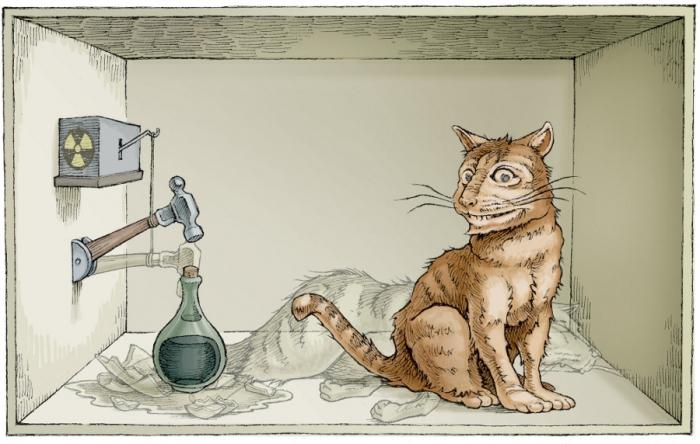
\includegraphics[width=90mm,scale=0.5]{catshred.jpg}
  \end{figure}
\end{frame}

\begin{frame}{Эксперимент Белла. Классический случай}
\[
f = \frac{1}{2}\left(
a b + a' b + a b' - a' b'
\right), a,a',b,b' \in \{-1, +1\}.
\]
следовательно
\(
f \in \{-1, +1\}
\)
и
\(
\left|\left<f\right>\right| \le 1
\)
\end{frame}

\begin{frame}{Эксперимент Белла. Квантовый случай}
\[
\left|\left<f\right>\right| = \sqrt{2} > 1
\]
\end{frame}


\begin{frame}{Отрицательные вероятности}
\[
\left<f\right> = \sum_{a,a',b,b'} p(a,a',b,b') f(a,a',b,b').
\]
следовательно для $\left|\left<f\right>\right| > 1$ необходимо
\[
\exists a,a',b,b': p(a,a',b,b') < 0
\]
\end{frame}

\section{Квантовые вычисления}
\begin{frame}{Классические вычисления}
\begin{figure}
\centering

\input ../part4/quantcomp/picclasscomp.tex

\caption{Классические вычисления. На вход подается число $x$ состоящее
  из $n$ бит, а на выходе имеем результат $y = f\left(x\right)$ описываемый $m$ битами}
\label{figQuantCompClassComp}
\end{figure}
\end{frame}

\begin{frame}{Квантовые вычисления}
\begin{figure}
\centering

\scalebox{.5}{%%Created by jPicEdt 1.5-pre1: mixed JPIC-XML/LaTeX format
%%Mon Oct 15 22:56:06 MSK 2012
%%Begin JPIC-XML
%<?xml version="1.0" standalone="yes"?>
%<jpic x-min="10" x-max="55" y-min="0" y-max="60" auto-bounding="true">
%<parallelogram p3="(40,0)"
%	 p2="(40,60)"
%	 p1="(20,60)"
%	 />
%<multicurve points="(10,55);(10,55);(20,55);(20,55)"
%	 />
%<multicurve points="(10,35);(10,35);(20,35);(20,35)"
%	 />
%<multicurve points="(10,25);(10,25);(20,25);(20,25)"
%	 />
%<multicurve points="(10,5);(10,5);(20,5);(20,5)"
%	 />
%<multicurve points="(40,55);(40,55);(50,55);(50,55)"
%	 />
%<multicurve points="(40,35);(40,35);(50,35);(50,35)"
%	 />
%<multicurve points="(40,25);(40,25);(50,25);(50,25)"
%	 />
%<multicurve points="(40,5);(40,5);(50,5);(50,5)"
%	 />
%<text stroke-style="dashed"
%	 stroke-dasharray="1;1"
%	 anchor-point="(10,15)"
%	 >
%$\left|0 \dots 0\right&gt;$
%</text>
%<text anchor-point="(25,55)"
%	 >
%$\hat{U}_f$
%</text>
%<text anchor-point="(10,45)"
%	 >
%$\left|x\right&gt;$
%</text>
%<text anchor-point="(45,45)"
%	 >
%$\left|x\right&gt;$
%</text>
%<text anchor-point="(55,15)"
%	 >
%$\left|y\right&gt; = \left|f\left(x\right)\right&gt;$
%</text>
%</jpic>
%%End JPIC-XML
%LaTeX-picture environment using emulated lines and arcs
%You can rescale the whole picture (to 80% for instance) by using the command \def\JPicScale{0.8}
\ifx\JPicScale\undefined\def\JPicScale{1}\fi
\unitlength \JPicScale mm
\begin{picture}(55,60)(0,0)
\linethickness{0.3mm}
\put(20,60){\line(1,0){20}}
\put(20,0){\line(0,1){60}}
\put(40,0){\line(0,1){60}}
\put(20,0){\line(1,0){20}}
\linethickness{0.3mm}
\put(10,55){\line(1,0){10}}
\linethickness{0.3mm}
\put(10,35){\line(1,0){10}}
\linethickness{0.3mm}
\put(10,25){\line(1,0){10}}
\linethickness{0.3mm}
\put(10,5){\line(1,0){10}}
\linethickness{0.3mm}
\put(40,55){\line(1,0){10}}
\linethickness{0.3mm}
\put(40,35){\line(1,0){10}}
\linethickness{0.3mm}
\put(40,25){\line(1,0){10}}
\linethickness{0.3mm}
\put(40,5){\line(1,0){10}}
\put(10,15){\makebox(0,0)[cc]{$\left|0 \dots 0\right>$}}

\put(25,55){\makebox(0,0)[cc]{$\hat{U}_f$}}

\put(10,45){\makebox(0,0)[cc]{$\ket{x}$}}

\put(45,45){\makebox(0,0)[cc]{$\ket{x}$}}

\put(55,15){\makebox(0,0)[cc]{$\ket{y} = \left|f\left(x\right)\right>$}}

\end{picture}
}

\caption{Квантовые обратимые вычисления. На вход подается число
  $\left|x\right>$ состоящее из $n$ кубит и затравка из нулевых
  состояний ($m$ кубит), а на выходе имеем результат $\left|y\right> =
  \left|f\left(x\right)\right>$ описываемый $m$ кубитами и исходное
  состояние $\left|x\right>$} 
\label{figQuantCompQuantComp}
\end{figure}
\end{frame}


\begin{frame}{Квантовые вычисления}
Классический случай
\[
x \to f(x)
\]
Квантовый случай
\begin{eqnarray}
\left|0\right>\left|0\right> + \left|1\right>\left|0\right> + \left|2\right>\left|0\right> +
\dots + \left|x\right>\left|0\right> + \dots \to
\nonumber \\
\to 
\left|0\right>\left|f(0)\right> + \left|1\right>\left|f(1)\right> + \left|2\right>\left|f(2)\right> +
\dots + \left|x\right>\left|f(x)\right> + \dots
\nonumber
\end{eqnarray}
\end{frame}


\section{Алгоритм Гровера}
\begin{frame}{Задача о поиске иголки в стоге сена}
\begin{figure}
\centering

\input ../part4/quantcomp/picsearch.tex

\caption{Поиск в неструктурированном объеме данных (поиск "иголки в
  стоге сена"). Классическая сложность $O(N)$}
\label{figQuantCompSearch}
\end{figure}
\end{frame}

\begin{frame}{Алгоритм Гровера. Схема}
\begin{figure}
\centering

\scalebox{.5}{%%Created by jPicEdt 1.5-pre1: mixed JPIC-XML/LaTeX format
%%Tue Jan 01 23:24:17 MSK 2013
%%Begin JPIC-XML
%<?xml version="1.0" standalone="yes"?>
%<jpic x-min="-1.67" x-max="80" y-min="0" y-max="35.71" auto-bounding="true">
%<parallelogram p3="(25,7.14)"
%	 p2="(25,35.71)"
%	 p1="(11.67,35.71)"
%	 />
%<parallelogram p3="(51.67,7.14)"
%	 p2="(51.67,35.71)"
%	 p1="(38.33,35.71)"
%	 />
%<multicurve right-arrow="head"
%	 points="(-1.67,21.43);(-1.67,21.43);(11.67,21.43);(11.67,21.43)"
%	 />
%<multicurve right-arrow="head"
%	 points="(25,21.43);(25,21.43);(38.33,21.43);(38.33,21.43)"
%	 />
%<multicurve right-arrow="head"
%	 points="(51.67,21.43);(51.67,21.43);(65,21.43);(65,21.43)"
%	 />
%<multicurve points="(58.33,21.43);(58.33,21.43);(58.33,0);(58.33,0)"
%	 />
%<multicurve points="(58.33,0);(58.33,0);(31.67,0);(31.67,0)"
%	 />
%<multicurve right-arrow="head"
%	 points="(31.67,0);(31.67,0);(31.67,21.43);(31.67,21.43)"
%	 />
%<text anchor-point="(20,30)"
%	 >
%$\hat{H}^{\otimes n}$
%</text>
%<text anchor-point="(45,30)"
%	 >
%$\hat{U}_G$
%</text>
%<ellipse p3="(80,25)"
%	 p2="(80,15)"
%	 p1="(70,15)"
%	 closure="open"
%	 angle-end="180"
%	 angle-start="0"
%	 />
%<multicurve right-arrow="head"
%	 points="(75,20);(75,20);(80,25);(80,25)"
%	 />
%</jpic>
%%End JPIC-XML
%LaTeX-picture environment using emulated lines and arcs
%You can rescale the whole picture (to 80% for instance) by using the command \def\JPicScale{0.8}
\ifx\JPicScale\undefined\def\JPicScale{1}\fi
\unitlength \JPicScale mm
\begin{picture}(80,35.71)(0,0)
\linethickness{0.3mm}
\put(11.67,35.71){\line(1,0){13.33}}
\put(11.67,7.14){\line(0,1){28.57}}
\put(25,7.14){\line(0,1){28.57}}
\put(11.67,7.14){\line(1,0){13.33}}
\linethickness{0.3mm}
\put(38.33,35.71){\line(1,0){13.34}}
\put(38.33,7.14){\line(0,1){28.57}}
\put(51.67,7.14){\line(0,1){28.57}}
\put(38.33,7.14){\line(1,0){13.34}}
\linethickness{0.3mm}
\put(-1.67,21.43){\line(1,0){13.34}}
\put(11.67,21.43){\vector(1,0){0.12}}
\linethickness{0.3mm}
\put(25,21.43){\line(1,0){13.33}}
\put(38.33,21.43){\vector(1,0){0.12}}
\linethickness{0.3mm}
\put(51.67,21.43){\line(1,0){13.33}}
\put(65,21.43){\vector(1,0){0.12}}
\linethickness{0.3mm}
\put(58.33,0){\line(0,1){21.43}}
\linethickness{0.3mm}
\put(31.67,0){\line(1,0){26.66}}
\linethickness{0.3mm}
\put(31.67,0){\line(0,1){21.43}}
\put(31.67,21.43){\vector(0,1){0.12}}
\put(20,30){\makebox(0,0)[cc]{$\hat{H}^{\otimes n}$}}

\put(45,30){\makebox(0,0)[cc]{$\hat{U}_G$}}

\linethickness{0.3mm}
\multiput(79.97,20.51)(0.03,-0.51){1}{\line(0,-1){0.51}}
\multiput(79.9,21.01)(0.08,-0.5){1}{\line(0,-1){0.5}}
\multiput(79.77,21.5)(0.13,-0.49){1}{\line(0,-1){0.49}}
\multiput(79.59,21.97)(0.18,-0.47){1}{\line(0,-1){0.47}}
\multiput(79.37,22.43)(0.11,-0.23){2}{\line(0,-1){0.23}}
\multiput(79.1,22.86)(0.13,-0.21){2}{\line(0,-1){0.21}}
\multiput(78.79,23.26)(0.1,-0.13){3}{\line(0,-1){0.13}}
\multiput(78.44,23.62)(0.12,-0.12){3}{\line(0,-1){0.12}}
\multiput(78.06,23.95)(0.13,-0.11){3}{\line(1,0){0.13}}
\multiput(77.64,24.24)(0.21,-0.14){2}{\line(1,0){0.21}}
\multiput(77.2,24.49)(0.22,-0.12){2}{\line(1,0){0.22}}
\multiput(76.74,24.69)(0.23,-0.1){2}{\line(1,0){0.23}}
\multiput(76.25,24.84)(0.48,-0.15){1}{\line(1,0){0.48}}
\multiput(75.76,24.94)(0.5,-0.1){1}{\line(1,0){0.5}}
\multiput(75.25,24.99)(0.5,-0.05){1}{\line(1,0){0.5}}
\put(74.75,24.99){\line(1,0){0.51}}
\multiput(74.24,24.94)(0.5,0.05){1}{\line(1,0){0.5}}
\multiput(73.75,24.84)(0.5,0.1){1}{\line(1,0){0.5}}
\multiput(73.26,24.69)(0.48,0.15){1}{\line(1,0){0.48}}
\multiput(72.8,24.49)(0.23,0.1){2}{\line(1,0){0.23}}
\multiput(72.36,24.24)(0.22,0.12){2}{\line(1,0){0.22}}
\multiput(71.94,23.95)(0.21,0.14){2}{\line(1,0){0.21}}
\multiput(71.56,23.62)(0.13,0.11){3}{\line(1,0){0.13}}
\multiput(71.21,23.26)(0.12,0.12){3}{\line(0,1){0.12}}
\multiput(70.9,22.86)(0.1,0.13){3}{\line(0,1){0.13}}
\multiput(70.63,22.43)(0.13,0.21){2}{\line(0,1){0.21}}
\multiput(70.41,21.97)(0.11,0.23){2}{\line(0,1){0.23}}
\multiput(70.23,21.5)(0.18,0.47){1}{\line(0,1){0.47}}
\multiput(70.1,21.01)(0.13,0.49){1}{\line(0,1){0.49}}
\multiput(70.03,20.51)(0.08,0.5){1}{\line(0,1){0.5}}
\multiput(70,20)(0.03,0.51){1}{\line(0,1){0.51}}

\linethickness{0.3mm}
\multiput(75,20)(0.12,0.12){42}{\line(1,0){0.12}}
\put(80,25){\vector(1,1){0.12}}
\end{picture}
}

\scalebox{.5}{%%Created by jPicEdt 1.5-pre1: mixed JPIC-XML/LaTeX format
%%Fri Jan 04 22:39:29 MSK 2013
%%Begin JPIC-XML
%<?xml version="1.0" standalone="yes"?>
%<jpic x-min="-1.67" x-max="65" y-min="0" y-max="45" auto-bounding="true">
%<parallelogram p3="(25,7.14)"
%	 p2="(25,35.71)"
%	 p1="(11.67,35.71)"
%	 />
%<parallelogram p3="(51.67,7.14)"
%	 p2="(51.67,35.71)"
%	 p1="(38.33,35.71)"
%	 />
%<multicurve right-arrow="head"
%	 points="(-1.67,21.43);(-1.67,21.43);(11.67,21.43);(11.67,21.43)"
%	 />
%<multicurve right-arrow="head"
%	 points="(25,21.43);(25,21.43);(38.33,21.43);(38.33,21.43)"
%	 />
%<multicurve right-arrow="head"
%	 points="(51.67,21.43);(51.67,21.43);(65,21.43);(65,21.43)"
%	 />
%<text anchor-point="(10,40)"
%	 >
%$\hat{U}_G$
%</text>
%<text anchor-point="(15,30)"
%	 >
%$\hat{U}_{x^{\ast}}$
%</text>
%<text anchor-point="(45,30)"
%	 >
%$\hat{U_s}$
%</text>
%<parallelogram p3="(55,45)"
%	 p2="(55,0)"
%	 p1="(5,0)"
%	 />
%</jpic>
%%End JPIC-XML
%LaTeX-picture environment using emulated lines and arcs
%You can rescale the whole picture (to 80% for instance) by using the command \def\JPicScale{0.8}
\ifx\JPicScale\undefined\def\JPicScale{1}\fi
\unitlength \JPicScale mm
\begin{picture}(65,45)(0,0)
\linethickness{0.3mm}
\put(11.67,35.71){\line(1,0){13.33}}
\put(11.67,7.14){\line(0,1){28.57}}
\put(25,7.14){\line(0,1){28.57}}
\put(11.67,7.14){\line(1,0){13.33}}
\linethickness{0.3mm}
\put(38.33,35.71){\line(1,0){13.34}}
\put(38.33,7.14){\line(0,1){28.57}}
\put(51.67,7.14){\line(0,1){28.57}}
\put(38.33,7.14){\line(1,0){13.34}}
\linethickness{0.3mm}
\put(-1.67,21.43){\line(1,0){13.34}}
\put(11.67,21.43){\vector(1,0){0.12}}
\linethickness{0.3mm}
\put(25,21.43){\line(1,0){13.33}}
\put(38.33,21.43){\vector(1,0){0.12}}
\linethickness{0.3mm}
\put(51.67,21.43){\line(1,0){13.33}}
\put(65,21.43){\vector(1,0){0.12}}
\put(10,40){\makebox(0,0)[cc]{$\hat{U}_G$}}

\put(15,30){\makebox(0,0)[cc]{$\hat{U}_{x^{\ast}}$}}

\put(45,30){\makebox(0,0)[cc]{$\hat{U}_s$}}

\linethickness{0.3mm}
\put(5,0){\line(1,0){50}}
\put(5,0){\line(0,1){45}}
\put(55,0){\line(0,1){45}}
\put(5,45){\line(1,0){50}}
\end{picture}
}

\caption{Алгоритм Гровера. Сложность $ O(\sqrt{N})$}
\label{figQuantCompGrover}
\end{figure}
\end{frame}

\begin{frame}{Алгоритм Гровера. Принцип работы}
\begin{figure}
\centering

\scalebox{.5}{%%Created by jPicEdt 1.5-pre1: mixed JPIC-XML/LaTeX format
%%Fri Jan 04 23:37:05 MSK 2013
%%Begin JPIC-XML
%<?xml version="1.0" standalone="yes"?>
%<jpic x-min="-5" x-max="75" y-min="0" y-max="60" auto-bounding="true">
%<multicurve right-arrow="head"
%	 points="(-5,10);(-5,10);(75,10);(75,10)"
%	 />
%<multicurve right-arrow="head"
%	 points="(-5,40);(-5,40);(75,40);(75,40)"
%	 />
%<multicurve left-arrow="head"
%	 points="(0,60);(0,60);(0,35);(0,35)"
%	 />
%<multicurve points="(10,50);(10,50);(10,40);(10,40)"
%	 />
%<multicurve points="(20,50);(20,50);(20,40);(20,40)"
%	 />
%<multicurve points="(60,50);(60,50);(60,40);(60,40)"
%	 />
%<multicurve points="(70,50);(70,50);(70,40);(70,40)"
%	 />
%<multicurve points="(40,50);(40,50);(40,40);(40,40)"
%	 />
%<multicurve points="(40,10);(40,10);(40,0);(40,0)"
%	 />
%<multicurve left-arrow="head"
%	 points="(0,30);(0,30);(0,5);(0,5)"
%	 />
%<multicurve points="(10,20);(10,20);(10,10);(10,10)"
%	 />
%<multicurve points="(20,20);(20,20);(20,10);(20,10)"
%	 />
%<multicurve points="(60,20);(60,20);(60,10);(60,10)"
%	 />
%<multicurve points="(70,20);(70,20);(70,10);(70,10)"
%	 />
%<text anchor-point="(75,35)"
%	 >
%$x$
%</text>
%<text anchor-point="(75,5)"
%	 >
%$x$
%</text>
%<text anchor-point="(-5,30)"
%	 >
%$\alpha_x$
%</text>
%<text anchor-point="(-5,60)"
%	 >
%$\alpha_x$
%</text>
%<text anchor-point="(40,35)"
%	 >
%$x^{\ast}$
%</text>
%<text anchor-point="(45,5)"
%	 >
%$x^{\ast}$
%</text>
%</jpic>
%%End JPIC-XML
%LaTeX-picture environment using emulated lines and arcs
%You can rescale the whole picture (to 80% for instance) by using the command \def\JPicScale{0.8}
\ifx\JPicScale\undefined\def\JPicScale{1}\fi
\unitlength \JPicScale mm
\begin{picture}(75,60)(0,0)
\linethickness{0.3mm}
\put(-5,10){\line(1,0){80}}
\put(75,10){\vector(1,0){0.12}}
\linethickness{0.3mm}
\put(-5,40){\line(1,0){80}}
\put(75,40){\vector(1,0){0.12}}
\linethickness{0.3mm}
\put(0,35){\line(0,1){25}}
\put(0,60){\vector(0,1){0.12}}
\linethickness{0.3mm}
\put(10,40){\line(0,1){10}}
\linethickness{0.3mm}
\put(20,40){\line(0,1){10}}
\linethickness{0.3mm}
\put(60,40){\line(0,1){10}}
\linethickness{0.3mm}
\put(70,40){\line(0,1){10}}
\linethickness{0.3mm}
\put(40,40){\line(0,1){10}}
\linethickness{0.3mm}
\put(40,0){\line(0,1){10}}
\linethickness{0.3mm}
\put(0,5){\line(0,1){25}}
\put(0,30){\vector(0,1){0.12}}
\linethickness{0.3mm}
\put(10,10){\line(0,1){10}}
\linethickness{0.3mm}
\put(20,10){\line(0,1){10}}
\linethickness{0.3mm}
\put(60,10){\line(0,1){10}}
\linethickness{0.3mm}
\put(70,10){\line(0,1){10}}
\put(75,35){\makebox(0,0)[cc]{$x$}}

\put(75,5){\makebox(0,0)[cc]{$x$}}

\put(-5,30){\makebox(0,0)[cc]{$\alpha_x$}}

\put(-5,60){\makebox(0,0)[cc]{$\alpha_x$}}

\put(40,35){\makebox(0,0)[cc]{$x^{\ast}$}}

\put(45,5){\makebox(0,0)[cc]{$x^{\ast}$}}

\end{picture}
}

\caption{Алгоритм Гровера. Инверсия фазы}
\label{figQuantCompGroverInv}
\end{figure}
\end{frame}

\begin{frame}{Алгоритм Гровера. Принцип работы}
\begin{figure}
\centering

\scalebox{.5}{%%Created by jPicEdt 1.5-pre1: mixed JPIC-XML/LaTeX format
%%Sat Jan 05 00:03:20 MSK 2013
%%Begin JPIC-XML
%<?xml version="1.0" standalone="yes"?>
%<jpic x-min="-5" x-max="80" y-min="5" y-max="70" auto-bounding="true">
%<multicurve right-arrow="head"
%	 points="(-5,10);(-5,10);(80,10);(80,10)"
%	 />
%<multicurve right-arrow="head"
%	 points="(-5,50);(-5,50);(80,50);(80,50)"
%	 />
%<multicurve left-arrow="head"
%	 points="(0,70);(0,70);(0,45);(0,45)"
%	 />
%<multicurve points="(10,60);(10,60);(10,50);(10,50)"
%	 />
%<multicurve points="(20,60);(20,60);(20,50);(20,50)"
%	 />
%<multicurve points="(60,60);(60,60);(60,50);(60,50)"
%	 />
%<multicurve points="(70,60);(70,60);(70,50);(70,50)"
%	 />
%<multicurve points="(40,40);(40,40);(40,50);(40,50)"
%	 />
%<multicurve points="(40,10);(40,10);(40,25);(40,25)"
%	 />
%<multicurve left-arrow="head"
%	 points="(0,30);(0,30);(0,5);(0,5)"
%	 />
%<multicurve points="(10,15);(10,15);(10,10);(10,10)"
%	 />
%<multicurve points="(20,15);(20,15);(20,10);(20,10)"
%	 />
%<multicurve points="(60,15);(60,15);(60,10);(60,10)"
%	 />
%<multicurve points="(70,15);(70,15);(70,10);(70,10)"
%	 />
%<text anchor-point="(80,45)"
%	 >
%$x$
%</text>
%<text anchor-point="(80,5)"
%	 >
%$x$
%</text>
%<text anchor-point="(-5,30)"
%	 >
%$\alpha_x$
%</text>
%<text anchor-point="(-5,70)"
%	 >
%$\alpha_x$
%</text>
%<text anchor-point="(45,45)"
%	 >
%$x^{\ast}$
%</text>
%<text anchor-point="(40,5)"
%	 >
%$x^{\ast}$
%</text>
%<multicurve stroke-style="dashed"
%	 stroke-dasharray="1;1"
%	 points="(-5,55);(-5,55);(75,55);(75,55)"
%	 />
%<text stroke-style="dotted"
%	 anchor-point="(80,55)"
%	 >
%$\mathcal{M}$
%</text>
%</jpic>
%%End JPIC-XML
%LaTeX-picture environment using emulated lines and arcs
%You can rescale the whole picture (to 80% for instance) by using the command \def\JPicScale{0.8}
\ifx\JPicScale\undefined\def\JPicScale{1}\fi
\unitlength \JPicScale mm
\begin{picture}(80,70)(0,0)
\linethickness{0.3mm}
\put(-5,10){\line(1,0){85}}
\put(80,10){\vector(1,0){0.12}}
\linethickness{0.3mm}
\put(-5,50){\line(1,0){85}}
\put(80,50){\vector(1,0){0.12}}
\linethickness{0.3mm}
\put(0,45){\line(0,1){25}}
\put(0,70){\vector(0,1){0.12}}
\linethickness{0.3mm}
\put(10,50){\line(0,1){10}}
\linethickness{0.3mm}
\put(20,50){\line(0,1){10}}
\linethickness{0.3mm}
\put(60,50){\line(0,1){10}}
\linethickness{0.3mm}
\put(70,50){\line(0,1){10}}
\linethickness{0.3mm}
\put(40,40){\line(0,1){10}}
\linethickness{0.3mm}
\put(40,10){\line(0,1){15}}
\linethickness{0.3mm}
\put(0,5){\line(0,1){25}}
\put(0,30){\vector(0,1){0.12}}
\linethickness{0.3mm}
\put(10,10){\line(0,1){5}}
\linethickness{0.3mm}
\put(20,10){\line(0,1){5}}
\linethickness{0.3mm}
\put(60,10){\line(0,1){5}}
\linethickness{0.3mm}
\put(70,10){\line(0,1){5}}
\put(80,45){\makebox(0,0)[cc]{$x$}}

\put(80,5){\makebox(0,0)[cc]{$x$}}

\put(-5,30){\makebox(0,0)[cc]{$\alpha_x$}}

\put(-5,70){\makebox(0,0)[cc]{$\alpha_x$}}

\put(45,45){\makebox(0,0)[cc]{$x^{\ast}$}}

\put(40,5){\makebox(0,0)[cc]{$x^{\ast}$}}

\linethickness{0.3mm}
\multiput(-5,57.5)(1.98,0){41}{\line(1,0){0.99}}
\put(80,57){\makebox(0,0)[cc]{$\mathcal{M}$}}

\multiput(-5,17.5)(1.98,0){41}{\line(1,0){0.99}}
\put(80,17){\makebox(0,0)[cc]{$\mathcal{M}$}}

\end{picture}
}

\caption{Алгоритм Гровера. Обращение относительно
  среднего.}
\label{figQuantCompGroverInvMiddle}
\end{figure}

\end{frame}


\begin{frame}{Влияние на рекомендации к использованию}
$O(N) \rightarrow O(\sqrt{N})$
ведет например к следующей рекомендации
$AES_{128} \rightarrow AES_{256}$
\end{frame}


\section{Алгоритм Шора}
\begin{frame}{Несимметричное шифрование}
\begin{itemize}
\item RSA и задача факторизации чисел
\item Diffie-Hellman и дискретный логарифм
\item Elliptic curve и дискретный логарифм
\end{itemize}
\end{frame}

\begin{frame}{RSA и задача о нахождении периода функций}
\[
N = p \cdot q
\]
\[
f\left(x, a\right) = a^x \mod N.
\]
Период функции $T = 2r$, т.е.
\begin{eqnarray}
a^{x+2r} \mod N = a^x \mod N,
\nonumber \\
a^{2r} \equiv 1 \mod N,
\nonumber \\
(a^r + 1)(a^r - 1)  \equiv 0 \mod N
\nonumber
\end{eqnarray}
\end{frame}

\begin{frame}{Алгоритм Шора}
\begin{figure}
\centering

\scalebox{.5}{%%Created by jPicEdt 1.5-pre1: mixed JPIC-XML/LaTeX format
%%Tue Oct 16 23:37:48 MSK 2012
%%Begin JPIC-XML
%<?xml version="1.0" standalone="yes"?>
%<jpic x-min="0" x-max="145" y-min="0" y-max="60" auto-bounding="true">
%<multicurve points="(0,5);(0,5);(10,5);(10,5)"
%	 />
%<multicurve points="(0,25);(0,25);(10,25);(10,25)"
%	 />
%<multicurve points="(0,35);(0,35);(10,35);(10,35)"
%	 />
%<multicurve points="(0,55);(0,55);(10,55);(10,55)"
%	 />
%<multicurve points="(25,55);(25,55);(40,55);(40,55)"
%	 />
%<multicurve points="(25,35);(25,35);(40,35);(40,35)"
%	 />
%<multicurve points="(10,25);(10,25);(40,25);(40,25)"
%	 />
%<multicurve points="(10,5);(10,5);(40,5);(40,5)"
%	 />
%<parallelogram p3="(60,0)"
%	 p2="(60,60)"
%	 p1="(40,60)"
%	 />
%<multicurve points="(60,25);(60,25);(75,25);(75,25)"
%	 />
%<multicurve points="(60,5);(60,5);(75,5);(75,5)"
%	 />
%<multicurve points="(60,55);(60,55);(95,55);(95,55)"
%	 />
%<multicurve points="(60,35);(60,35);(95,35);(95,35)"
%	 />
%<multicurve points="(110,55);(110,55);(120,55);(120,55)"
%	 />
%<multicurve points="(110,35);(110,35);(120,35);(120,35)"
%	 />
%<ellipse p3="(145,50)"
%	 p2="(145,40)"
%	 p1="(135,40)"
%	 closure="open"
%	 angle-end="180"
%	 angle-start="0"
%	 />
%<multicurve right-arrow="head"
%	 points="(140,45);(140,45);(145,50);(145,50)"
%	 />
%<text anchor-point="(0,45)"
%	 >
%$\left|0\right&gt;$
%</text>
%<text anchor-point="(0,15)"
%	 >
%$\left|0\right&gt;$
%</text>
%<parallelogram p3="(25,30)"
%	 p2="(25,60)"
%	 p1="(10,60)"
%	 />
%<parallelogram p3="(110,30)"
%	 p2="(110,60)"
%	 p1="(95,60)"
%	 />
%<text anchor-point="(45,55)"
%	 >
%$\hat{U}_f$
%</text>
%<text anchor-point="(30,45)"
%	 >
%$\left|x\right&gt;$
%</text>
%<text anchor-point="(65,45)"
%	 >
%$\left|x\right&gt;$
%</text>
%<text anchor-point="(70,15)"
%	 >
%$\left|f\left(x\right)\right&gt;$
%</text>
%<text anchor-point="(85,45)"
%	 >
%$\left|x'\right&gt;$
%</text>
%<text anchor-point="(120,45)"
%	 >
%$\left|\tilde{X'}\right&gt;$
%</text>
%<text anchor-point="(100,55)"
%	 >
%$\hat{F}^M$
%</text>
%<ellipse p3="(100,20)"
%	 p2="(100,10)"
%	 p1="(90,10)"
%	 closure="open"
%	 angle-end="180"
%	 angle-start="0"
%	 />
%<multicurve right-arrow="head"
%	 points="(95,15);(95,15);(100,20);(100,20)"
%	 />
%<text anchor-point="(15,55)"
%	 >
%$\hat{H}^{\otimes n}$
%</text>
%</jpic>
%%End JPIC-XML
%LaTeX-picture environment using emulated lines and arcs
%You can rescale the whole picture (to 80% for instance) by using the command \def\JPicScale{0.8}
\ifx\JPicScale\undefined\def\JPicScale{1}\fi
\unitlength \JPicScale mm
\begin{picture}(145,60)(0,0)
\linethickness{0.3mm}
\put(0,5){\line(1,0){10}}
\linethickness{0.3mm}
\put(0,25){\line(1,0){10}}
\linethickness{0.3mm}
\put(0,35){\line(1,0){10}}
\linethickness{0.3mm}
\put(0,55){\line(1,0){10}}
\linethickness{0.3mm}
\put(25,55){\line(1,0){15}}
\linethickness{0.3mm}
\put(25,35){\line(1,0){15}}
\linethickness{0.3mm}
\put(10,25){\line(1,0){30}}
\linethickness{0.3mm}
\put(10,5){\line(1,0){30}}
\linethickness{0.3mm}
\put(40,60){\line(1,0){20}}
\put(40,0){\line(0,1){60}}
\put(60,0){\line(0,1){60}}
\put(40,0){\line(1,0){20}}
\linethickness{0.3mm}
\put(60,25){\line(1,0){15}}
\linethickness{0.3mm}
\put(60,5){\line(1,0){15}}
\linethickness{0.3mm}
\put(60,55){\line(1,0){35}}
\linethickness{0.3mm}
\put(60,35){\line(1,0){35}}
\linethickness{0.3mm}
\put(110,55){\line(1,0){10}}
\linethickness{0.3mm}
\put(110,35){\line(1,0){10}}
\linethickness{0.3mm}
\multiput(144.97,45.51)(0.03,-0.51){1}{\line(0,-1){0.51}}
\multiput(144.9,46.01)(0.08,-0.5){1}{\line(0,-1){0.5}}
\multiput(144.77,46.5)(0.13,-0.49){1}{\line(0,-1){0.49}}
\multiput(144.59,46.97)(0.18,-0.47){1}{\line(0,-1){0.47}}
\multiput(144.37,47.43)(0.11,-0.23){2}{\line(0,-1){0.23}}
\multiput(144.1,47.86)(0.13,-0.21){2}{\line(0,-1){0.21}}
\multiput(143.79,48.26)(0.1,-0.13){3}{\line(0,-1){0.13}}
\multiput(143.44,48.62)(0.12,-0.12){3}{\line(0,-1){0.12}}
\multiput(143.06,48.95)(0.13,-0.11){3}{\line(1,0){0.13}}
\multiput(142.64,49.24)(0.21,-0.14){2}{\line(1,0){0.21}}
\multiput(142.2,49.49)(0.22,-0.12){2}{\line(1,0){0.22}}
\multiput(141.74,49.69)(0.23,-0.1){2}{\line(1,0){0.23}}
\multiput(141.25,49.84)(0.48,-0.15){1}{\line(1,0){0.48}}
\multiput(140.76,49.94)(0.5,-0.1){1}{\line(1,0){0.5}}
\multiput(140.25,49.99)(0.5,-0.05){1}{\line(1,0){0.5}}
\put(139.75,49.99){\line(1,0){0.51}}
\multiput(139.24,49.94)(0.5,0.05){1}{\line(1,0){0.5}}
\multiput(138.75,49.84)(0.5,0.1){1}{\line(1,0){0.5}}
\multiput(138.26,49.69)(0.48,0.15){1}{\line(1,0){0.48}}
\multiput(137.8,49.49)(0.23,0.1){2}{\line(1,0){0.23}}
\multiput(137.36,49.24)(0.22,0.12){2}{\line(1,0){0.22}}
\multiput(136.94,48.95)(0.21,0.14){2}{\line(1,0){0.21}}
\multiput(136.56,48.62)(0.13,0.11){3}{\line(1,0){0.13}}
\multiput(136.21,48.26)(0.12,0.12){3}{\line(0,1){0.12}}
\multiput(135.9,47.86)(0.1,0.13){3}{\line(0,1){0.13}}
\multiput(135.63,47.43)(0.13,0.21){2}{\line(0,1){0.21}}
\multiput(135.41,46.97)(0.11,0.23){2}{\line(0,1){0.23}}
\multiput(135.23,46.5)(0.18,0.47){1}{\line(0,1){0.47}}
\multiput(135.1,46.01)(0.13,0.49){1}{\line(0,1){0.49}}
\multiput(135.03,45.51)(0.08,0.5){1}{\line(0,1){0.5}}
\multiput(135,45)(0.03,0.51){1}{\line(0,1){0.51}}

\linethickness{0.3mm}
\multiput(140,45)(0.12,0.12){42}{\line(1,0){0.12}}
\put(145,50){\vector(1,1){0.12}}
\put(0,45){\makebox(0,0)[cc]{$\left|0\right>$}}

\put(0,15){\makebox(0,0)[cc]{$\left|0\right>$}}

\linethickness{0.3mm}
\put(10,60){\line(1,0){15}}
\put(10,30){\line(0,1){30}}
\put(25,30){\line(0,1){30}}
\put(10,30){\line(1,0){15}}
\linethickness{0.3mm}
\put(95,60){\line(1,0){15}}
\put(95,30){\line(0,1){30}}
\put(110,30){\line(0,1){30}}
\put(95,30){\line(1,0){15}}
\put(45,55){\makebox(0,0)[cc]{$\hat{U}_f$}}

\put(30,45){\makebox(0,0)[cc]{$\left|x\right>$}}

\put(65,45){\makebox(0,0)[cc]{$\left|x\right>$}}

\put(70,15){\makebox(0,0)[cc]{$\left|f\left(x\right)\right>$}}

\put(85,45){\makebox(0,0)[cc]{$\left|x'\right>$}}

\put(120,45){\makebox(0,0)[cc]{$\left|\tilde{X'}\right>$}}

\put(100,55){\makebox(0,0)[cc]{$\hat{F}^M$}}

\linethickness{0.3mm}
\multiput(99.97,15.51)(0.03,-0.51){1}{\line(0,-1){0.51}}
\multiput(99.9,16.01)(0.08,-0.5){1}{\line(0,-1){0.5}}
\multiput(99.77,16.5)(0.13,-0.49){1}{\line(0,-1){0.49}}
\multiput(99.59,16.97)(0.18,-0.47){1}{\line(0,-1){0.47}}
\multiput(99.37,17.43)(0.11,-0.23){2}{\line(0,-1){0.23}}
\multiput(99.1,17.86)(0.13,-0.21){2}{\line(0,-1){0.21}}
\multiput(98.79,18.26)(0.1,-0.13){3}{\line(0,-1){0.13}}
\multiput(98.44,18.62)(0.12,-0.12){3}{\line(0,-1){0.12}}
\multiput(98.06,18.95)(0.13,-0.11){3}{\line(1,0){0.13}}
\multiput(97.64,19.24)(0.21,-0.14){2}{\line(1,0){0.21}}
\multiput(97.2,19.49)(0.22,-0.12){2}{\line(1,0){0.22}}
\multiput(96.74,19.69)(0.23,-0.1){2}{\line(1,0){0.23}}
\multiput(96.25,19.84)(0.48,-0.15){1}{\line(1,0){0.48}}
\multiput(95.76,19.94)(0.5,-0.1){1}{\line(1,0){0.5}}
\multiput(95.25,19.99)(0.5,-0.05){1}{\line(1,0){0.5}}
\put(94.75,19.99){\line(1,0){0.51}}
\multiput(94.24,19.94)(0.5,0.05){1}{\line(1,0){0.5}}
\multiput(93.75,19.84)(0.5,0.1){1}{\line(1,0){0.5}}
\multiput(93.26,19.69)(0.48,0.15){1}{\line(1,0){0.48}}
\multiput(92.8,19.49)(0.23,0.1){2}{\line(1,0){0.23}}
\multiput(92.36,19.24)(0.22,0.12){2}{\line(1,0){0.22}}
\multiput(91.94,18.95)(0.21,0.14){2}{\line(1,0){0.21}}
\multiput(91.56,18.62)(0.13,0.11){3}{\line(1,0){0.13}}
\multiput(91.21,18.26)(0.12,0.12){3}{\line(0,1){0.12}}
\multiput(90.9,17.86)(0.1,0.13){3}{\line(0,1){0.13}}
\multiput(90.63,17.43)(0.13,0.21){2}{\line(0,1){0.21}}
\multiput(90.41,16.97)(0.11,0.23){2}{\line(0,1){0.23}}
\multiput(90.23,16.5)(0.18,0.47){1}{\line(0,1){0.47}}
\multiput(90.1,16.01)(0.13,0.49){1}{\line(0,1){0.49}}
\multiput(90.03,15.51)(0.08,0.5){1}{\line(0,1){0.5}}
\multiput(90,15)(0.03,0.51){1}{\line(0,1){0.51}}

\linethickness{0.3mm}
\multiput(95,15)(0.12,0.12){42}{\line(1,0){0.12}}
\put(100,20){\vector(1,1){0.12}}
\put(15,55){\makebox(0,0)[cc]{$\hat{H}^{\otimes n}$}}

\end{picture}
}

\caption{ Определение периода функций с помощью квантового
  преобразования Фурье}
\end{figure}
\end{frame}


\begin{frame}{Алгоритм Шора. Нахождение периода функции 
  $f\left(x, a\right) = a^x \mod{N}$}
\begin{figure}
\centering

\scalebox{.5}{% GNUPLOT: LaTeX picture
\setlength{\unitlength}{0.240900pt}
\ifx\plotpoint\undefined\newsavebox{\plotpoint}\fi
\begin{picture}(1500,900)(0,0)
\sbox{\plotpoint}{\rule[-0.200pt]{0.400pt}{0.400pt}}%
\put(151.0,131.0){\rule[-0.200pt]{4.818pt}{0.400pt}}
\put(131,131){\makebox(0,0)[r]{ 0}}
\put(1419.0,131.0){\rule[-0.200pt]{4.818pt}{0.400pt}}
\put(151.0,212.0){\rule[-0.200pt]{4.818pt}{0.400pt}}
\put(131,212){\makebox(0,0)[r]{ 2}}
\put(1419.0,212.0){\rule[-0.200pt]{4.818pt}{0.400pt}}
\put(151.0,293.0){\rule[-0.200pt]{4.818pt}{0.400pt}}
\put(131,293){\makebox(0,0)[r]{ 4}}
\put(1419.0,293.0){\rule[-0.200pt]{4.818pt}{0.400pt}}
\put(151.0,374.0){\rule[-0.200pt]{4.818pt}{0.400pt}}
\put(131,374){\makebox(0,0)[r]{ 6}}
\put(1419.0,374.0){\rule[-0.200pt]{4.818pt}{0.400pt}}
\put(151.0,455.0){\rule[-0.200pt]{4.818pt}{0.400pt}}
\put(131,455){\makebox(0,0)[r]{ 8}}
\put(1419.0,455.0){\rule[-0.200pt]{4.818pt}{0.400pt}}
\put(151.0,535.0){\rule[-0.200pt]{4.818pt}{0.400pt}}
\put(131,535){\makebox(0,0)[r]{ 10}}
\put(1419.0,535.0){\rule[-0.200pt]{4.818pt}{0.400pt}}
\put(151.0,616.0){\rule[-0.200pt]{4.818pt}{0.400pt}}
\put(131,616){\makebox(0,0)[r]{ 12}}
\put(1419.0,616.0){\rule[-0.200pt]{4.818pt}{0.400pt}}
\put(151.0,697.0){\rule[-0.200pt]{4.818pt}{0.400pt}}
\put(131,697){\makebox(0,0)[r]{ 14}}
\put(1419.0,697.0){\rule[-0.200pt]{4.818pt}{0.400pt}}
\put(151.0,778.0){\rule[-0.200pt]{4.818pt}{0.400pt}}
\put(131,778){\makebox(0,0)[r]{ 16}}
\put(1419.0,778.0){\rule[-0.200pt]{4.818pt}{0.400pt}}
\put(151.0,859.0){\rule[-0.200pt]{4.818pt}{0.400pt}}
\put(131,859){\makebox(0,0)[r]{ 18}}
\put(1419.0,859.0){\rule[-0.200pt]{4.818pt}{0.400pt}}
\put(335.0,131.0){\rule[-0.200pt]{0.400pt}{4.818pt}}
\put(335,90){\makebox(0,0){ 10}}
\put(335.0,839.0){\rule[-0.200pt]{0.400pt}{4.818pt}}
\put(539.0,131.0){\rule[-0.200pt]{0.400pt}{4.818pt}}
\put(539,90){\makebox(0,0){ 20}}
\put(539.0,839.0){\rule[-0.200pt]{0.400pt}{4.818pt}}
\put(744.0,131.0){\rule[-0.200pt]{0.400pt}{4.818pt}}
\put(744,90){\makebox(0,0){ 30}}
\put(744.0,839.0){\rule[-0.200pt]{0.400pt}{4.818pt}}
\put(948.0,131.0){\rule[-0.200pt]{0.400pt}{4.818pt}}
\put(948,90){\makebox(0,0){ 40}}
\put(948.0,839.0){\rule[-0.200pt]{0.400pt}{4.818pt}}
\put(1153.0,131.0){\rule[-0.200pt]{0.400pt}{4.818pt}}
\put(1153,90){\makebox(0,0){ 50}}
\put(1153.0,839.0){\rule[-0.200pt]{0.400pt}{4.818pt}}
\put(1357.0,131.0){\rule[-0.200pt]{0.400pt}{4.818pt}}
\put(1357,90){\makebox(0,0){ 60}}
\put(1357.0,839.0){\rule[-0.200pt]{0.400pt}{4.818pt}}
\put(151.0,131.0){\rule[-0.200pt]{0.400pt}{175.375pt}}
\put(151.0,131.0){\rule[-0.200pt]{310.279pt}{0.400pt}}
\put(1439.0,131.0){\rule[-0.200pt]{0.400pt}{175.375pt}}
\put(151.0,859.0){\rule[-0.200pt]{310.279pt}{0.400pt}}
\put(30,495){\makebox(0,0){$f(x)$}}
\put(795,29){\makebox(0,0){$x$}}
\put(151,212){\usebox{\plotpoint}}
\multiput(151.58,212.00)(0.496,2.052){37}{\rule{0.119pt}{1.720pt}}
\multiput(150.17,212.00)(20.000,77.430){2}{\rule{0.400pt}{0.860pt}}
\multiput(171.58,293.00)(0.496,3.915){39}{\rule{0.119pt}{3.186pt}}
\multiput(170.17,293.00)(21.000,155.388){2}{\rule{0.400pt}{1.593pt}}
\multiput(192.58,455.00)(0.496,8.216){37}{\rule{0.119pt}{6.560pt}}
\multiput(191.17,455.00)(20.000,309.384){2}{\rule{0.400pt}{3.280pt}}
\multiput(212.58,761.61)(0.496,-4.885){39}{\rule{0.119pt}{3.948pt}}
\multiput(211.17,769.81)(21.000,-193.807){2}{\rule{0.400pt}{1.974pt}}
\multiput(233.58,541.96)(0.496,-10.304){37}{\rule{0.119pt}{8.200pt}}
\multiput(232.17,558.98)(20.000,-387.980){2}{\rule{0.400pt}{4.100pt}}
\multiput(253.58,171.00)(0.496,0.983){39}{\rule{0.119pt}{0.881pt}}
\multiput(252.17,171.00)(21.000,39.172){2}{\rule{0.400pt}{0.440pt}}
\multiput(274.58,212.00)(0.496,2.052){37}{\rule{0.119pt}{1.720pt}}
\multiput(273.17,212.00)(20.000,77.430){2}{\rule{0.400pt}{0.860pt}}
\multiput(294.58,293.00)(0.496,3.915){39}{\rule{0.119pt}{3.186pt}}
\multiput(293.17,293.00)(21.000,155.388){2}{\rule{0.400pt}{1.593pt}}
\multiput(315.58,455.00)(0.496,8.216){37}{\rule{0.119pt}{6.560pt}}
\multiput(314.17,455.00)(20.000,309.384){2}{\rule{0.400pt}{3.280pt}}
\multiput(335.58,760.81)(0.496,-5.134){37}{\rule{0.119pt}{4.140pt}}
\multiput(334.17,769.41)(20.000,-193.407){2}{\rule{0.400pt}{2.070pt}}
\multiput(355.58,543.56)(0.496,-9.804){39}{\rule{0.119pt}{7.814pt}}
\multiput(354.17,559.78)(21.000,-388.781){2}{\rule{0.400pt}{3.907pt}}
\multiput(376.58,171.00)(0.496,1.033){37}{\rule{0.119pt}{0.920pt}}
\multiput(375.17,171.00)(20.000,39.090){2}{\rule{0.400pt}{0.460pt}}
\multiput(396.58,212.00)(0.496,1.952){39}{\rule{0.119pt}{1.643pt}}
\multiput(395.17,212.00)(21.000,77.590){2}{\rule{0.400pt}{0.821pt}}
\multiput(417.58,293.00)(0.496,4.115){37}{\rule{0.119pt}{3.340pt}}
\multiput(416.17,293.00)(20.000,155.068){2}{\rule{0.400pt}{1.670pt}}
\multiput(437.58,455.00)(0.496,7.817){39}{\rule{0.119pt}{6.252pt}}
\multiput(436.17,455.00)(21.000,310.023){2}{\rule{0.400pt}{3.126pt}}
\multiput(458.58,760.81)(0.496,-5.134){37}{\rule{0.119pt}{4.140pt}}
\multiput(457.17,769.41)(20.000,-193.407){2}{\rule{0.400pt}{2.070pt}}
\multiput(478.58,543.56)(0.496,-9.804){39}{\rule{0.119pt}{7.814pt}}
\multiput(477.17,559.78)(21.000,-388.781){2}{\rule{0.400pt}{3.907pt}}
\multiput(499.58,171.00)(0.496,1.033){37}{\rule{0.119pt}{0.920pt}}
\multiput(498.17,171.00)(20.000,39.090){2}{\rule{0.400pt}{0.460pt}}
\multiput(519.58,212.00)(0.496,2.052){37}{\rule{0.119pt}{1.720pt}}
\multiput(518.17,212.00)(20.000,77.430){2}{\rule{0.400pt}{0.860pt}}
\multiput(539.58,293.00)(0.496,3.915){39}{\rule{0.119pt}{3.186pt}}
\multiput(538.17,293.00)(21.000,155.388){2}{\rule{0.400pt}{1.593pt}}
\multiput(560.58,455.00)(0.496,8.216){37}{\rule{0.119pt}{6.560pt}}
\multiput(559.17,455.00)(20.000,309.384){2}{\rule{0.400pt}{3.280pt}}
\multiput(580.58,761.61)(0.496,-4.885){39}{\rule{0.119pt}{3.948pt}}
\multiput(579.17,769.81)(21.000,-193.807){2}{\rule{0.400pt}{1.974pt}}
\multiput(601.58,541.96)(0.496,-10.304){37}{\rule{0.119pt}{8.200pt}}
\multiput(600.17,558.98)(20.000,-387.980){2}{\rule{0.400pt}{4.100pt}}
\multiput(621.58,171.00)(0.496,0.983){39}{\rule{0.119pt}{0.881pt}}
\multiput(620.17,171.00)(21.000,39.172){2}{\rule{0.400pt}{0.440pt}}
\multiput(642.58,212.00)(0.496,2.052){37}{\rule{0.119pt}{1.720pt}}
\multiput(641.17,212.00)(20.000,77.430){2}{\rule{0.400pt}{0.860pt}}
\multiput(662.58,293.00)(0.496,3.915){39}{\rule{0.119pt}{3.186pt}}
\multiput(661.17,293.00)(21.000,155.388){2}{\rule{0.400pt}{1.593pt}}
\multiput(683.58,455.00)(0.496,8.216){37}{\rule{0.119pt}{6.560pt}}
\multiput(682.17,455.00)(20.000,309.384){2}{\rule{0.400pt}{3.280pt}}
\multiput(703.58,760.81)(0.496,-5.134){37}{\rule{0.119pt}{4.140pt}}
\multiput(702.17,769.41)(20.000,-193.407){2}{\rule{0.400pt}{2.070pt}}
\multiput(723.58,543.56)(0.496,-9.804){39}{\rule{0.119pt}{7.814pt}}
\multiput(722.17,559.78)(21.000,-388.781){2}{\rule{0.400pt}{3.907pt}}
\multiput(744.58,171.00)(0.496,1.033){37}{\rule{0.119pt}{0.920pt}}
\multiput(743.17,171.00)(20.000,39.090){2}{\rule{0.400pt}{0.460pt}}
\multiput(764.58,212.00)(0.496,1.952){39}{\rule{0.119pt}{1.643pt}}
\multiput(763.17,212.00)(21.000,77.590){2}{\rule{0.400pt}{0.821pt}}
\multiput(785.58,293.00)(0.496,4.115){37}{\rule{0.119pt}{3.340pt}}
\multiput(784.17,293.00)(20.000,155.068){2}{\rule{0.400pt}{1.670pt}}
\multiput(805.58,455.00)(0.496,7.817){39}{\rule{0.119pt}{6.252pt}}
\multiput(804.17,455.00)(21.000,310.023){2}{\rule{0.400pt}{3.126pt}}
\multiput(826.58,760.81)(0.496,-5.134){37}{\rule{0.119pt}{4.140pt}}
\multiput(825.17,769.41)(20.000,-193.407){2}{\rule{0.400pt}{2.070pt}}
\multiput(846.58,543.56)(0.496,-9.804){39}{\rule{0.119pt}{7.814pt}}
\multiput(845.17,559.78)(21.000,-388.781){2}{\rule{0.400pt}{3.907pt}}
\multiput(867.58,171.00)(0.496,1.033){37}{\rule{0.119pt}{0.920pt}}
\multiput(866.17,171.00)(20.000,39.090){2}{\rule{0.400pt}{0.460pt}}
\multiput(887.58,212.00)(0.496,2.052){37}{\rule{0.119pt}{1.720pt}}
\multiput(886.17,212.00)(20.000,77.430){2}{\rule{0.400pt}{0.860pt}}
\multiput(907.58,293.00)(0.496,3.915){39}{\rule{0.119pt}{3.186pt}}
\multiput(906.17,293.00)(21.000,155.388){2}{\rule{0.400pt}{1.593pt}}
\multiput(928.58,455.00)(0.496,8.216){37}{\rule{0.119pt}{6.560pt}}
\multiput(927.17,455.00)(20.000,309.384){2}{\rule{0.400pt}{3.280pt}}
\multiput(948.58,761.61)(0.496,-4.885){39}{\rule{0.119pt}{3.948pt}}
\multiput(947.17,769.81)(21.000,-193.807){2}{\rule{0.400pt}{1.974pt}}
\multiput(969.58,541.96)(0.496,-10.304){37}{\rule{0.119pt}{8.200pt}}
\multiput(968.17,558.98)(20.000,-387.980){2}{\rule{0.400pt}{4.100pt}}
\multiput(989.58,171.00)(0.496,0.983){39}{\rule{0.119pt}{0.881pt}}
\multiput(988.17,171.00)(21.000,39.172){2}{\rule{0.400pt}{0.440pt}}
\multiput(1010.58,212.00)(0.496,2.052){37}{\rule{0.119pt}{1.720pt}}
\multiput(1009.17,212.00)(20.000,77.430){2}{\rule{0.400pt}{0.860pt}}
\multiput(1030.58,293.00)(0.496,3.915){39}{\rule{0.119pt}{3.186pt}}
\multiput(1029.17,293.00)(21.000,155.388){2}{\rule{0.400pt}{1.593pt}}
\multiput(1051.58,455.00)(0.496,8.216){37}{\rule{0.119pt}{6.560pt}}
\multiput(1050.17,455.00)(20.000,309.384){2}{\rule{0.400pt}{3.280pt}}
\multiput(1071.58,760.81)(0.496,-5.134){37}{\rule{0.119pt}{4.140pt}}
\multiput(1070.17,769.41)(20.000,-193.407){2}{\rule{0.400pt}{2.070pt}}
\multiput(1091.58,543.56)(0.496,-9.804){39}{\rule{0.119pt}{7.814pt}}
\multiput(1090.17,559.78)(21.000,-388.781){2}{\rule{0.400pt}{3.907pt}}
\multiput(1112.58,171.00)(0.496,1.033){37}{\rule{0.119pt}{0.920pt}}
\multiput(1111.17,171.00)(20.000,39.090){2}{\rule{0.400pt}{0.460pt}}
\multiput(1132.58,212.00)(0.496,1.952){39}{\rule{0.119pt}{1.643pt}}
\multiput(1131.17,212.00)(21.000,77.590){2}{\rule{0.400pt}{0.821pt}}
\multiput(1153.58,293.00)(0.496,4.115){37}{\rule{0.119pt}{3.340pt}}
\multiput(1152.17,293.00)(20.000,155.068){2}{\rule{0.400pt}{1.670pt}}
\multiput(1173.58,455.00)(0.496,7.817){39}{\rule{0.119pt}{6.252pt}}
\multiput(1172.17,455.00)(21.000,310.023){2}{\rule{0.400pt}{3.126pt}}
\multiput(1194.58,760.81)(0.496,-5.134){37}{\rule{0.119pt}{4.140pt}}
\multiput(1193.17,769.41)(20.000,-193.407){2}{\rule{0.400pt}{2.070pt}}
\multiput(1214.58,543.56)(0.496,-9.804){39}{\rule{0.119pt}{7.814pt}}
\multiput(1213.17,559.78)(21.000,-388.781){2}{\rule{0.400pt}{3.907pt}}
\multiput(1235.58,171.00)(0.496,1.033){37}{\rule{0.119pt}{0.920pt}}
\multiput(1234.17,171.00)(20.000,39.090){2}{\rule{0.400pt}{0.460pt}}
\multiput(1255.58,212.00)(0.496,2.052){37}{\rule{0.119pt}{1.720pt}}
\multiput(1254.17,212.00)(20.000,77.430){2}{\rule{0.400pt}{0.860pt}}
\multiput(1275.58,293.00)(0.496,3.915){39}{\rule{0.119pt}{3.186pt}}
\multiput(1274.17,293.00)(21.000,155.388){2}{\rule{0.400pt}{1.593pt}}
\multiput(1296.58,455.00)(0.496,8.216){37}{\rule{0.119pt}{6.560pt}}
\multiput(1295.17,455.00)(20.000,309.384){2}{\rule{0.400pt}{3.280pt}}
\multiput(1316.58,761.61)(0.496,-4.885){39}{\rule{0.119pt}{3.948pt}}
\multiput(1315.17,769.81)(21.000,-193.807){2}{\rule{0.400pt}{1.974pt}}
\multiput(1337.58,541.96)(0.496,-10.304){37}{\rule{0.119pt}{8.200pt}}
\multiput(1336.17,558.98)(20.000,-387.980){2}{\rule{0.400pt}{4.100pt}}
\multiput(1357.58,171.00)(0.496,0.983){39}{\rule{0.119pt}{0.881pt}}
\multiput(1356.17,171.00)(21.000,39.172){2}{\rule{0.400pt}{0.440pt}}
\multiput(1378.58,212.00)(0.496,2.052){37}{\rule{0.119pt}{1.720pt}}
\multiput(1377.17,212.00)(20.000,77.430){2}{\rule{0.400pt}{0.860pt}}
\multiput(1398.58,293.00)(0.496,3.915){39}{\rule{0.119pt}{3.186pt}}
\multiput(1397.17,293.00)(21.000,155.388){2}{\rule{0.400pt}{1.593pt}}
\multiput(1419.58,455.00)(0.496,8.216){37}{\rule{0.119pt}{6.560pt}}
\multiput(1418.17,455.00)(20.000,309.384){2}{\rule{0.400pt}{3.280pt}}
\put(151,212){\makebox(0,0){$\bullet$}}
\put(171,293){\makebox(0,0){$\bullet$}}
\put(192,455){\makebox(0,0){$\bullet$}}
\put(212,778){\makebox(0,0){$\bullet$}}
\put(233,576){\makebox(0,0){$\bullet$}}
\put(253,171){\makebox(0,0){$\bullet$}}
\put(274,212){\makebox(0,0){$\bullet$}}
\put(294,293){\makebox(0,0){$\bullet$}}
\put(315,455){\makebox(0,0){$\bullet$}}
\put(335,778){\makebox(0,0){$\bullet$}}
\put(355,576){\makebox(0,0){$\bullet$}}
\put(376,171){\makebox(0,0){$\bullet$}}
\put(396,212){\makebox(0,0){$\bullet$}}
\put(417,293){\makebox(0,0){$\bullet$}}
\put(437,455){\makebox(0,0){$\bullet$}}
\put(458,778){\makebox(0,0){$\bullet$}}
\put(478,576){\makebox(0,0){$\bullet$}}
\put(499,171){\makebox(0,0){$\bullet$}}
\put(519,212){\makebox(0,0){$\bullet$}}
\put(539,293){\makebox(0,0){$\bullet$}}
\put(560,455){\makebox(0,0){$\bullet$}}
\put(580,778){\makebox(0,0){$\bullet$}}
\put(601,576){\makebox(0,0){$\bullet$}}
\put(621,171){\makebox(0,0){$\bullet$}}
\put(642,212){\makebox(0,0){$\bullet$}}
\put(662,293){\makebox(0,0){$\bullet$}}
\put(683,455){\makebox(0,0){$\bullet$}}
\put(703,778){\makebox(0,0){$\bullet$}}
\put(723,576){\makebox(0,0){$\bullet$}}
\put(744,171){\makebox(0,0){$\bullet$}}
\put(764,212){\makebox(0,0){$\bullet$}}
\put(785,293){\makebox(0,0){$\bullet$}}
\put(805,455){\makebox(0,0){$\bullet$}}
\put(826,778){\makebox(0,0){$\bullet$}}
\put(846,576){\makebox(0,0){$\bullet$}}
\put(867,171){\makebox(0,0){$\bullet$}}
\put(887,212){\makebox(0,0){$\bullet$}}
\put(907,293){\makebox(0,0){$\bullet$}}
\put(928,455){\makebox(0,0){$\bullet$}}
\put(948,778){\makebox(0,0){$\bullet$}}
\put(969,576){\makebox(0,0){$\bullet$}}
\put(989,171){\makebox(0,0){$\bullet$}}
\put(1010,212){\makebox(0,0){$\bullet$}}
\put(1030,293){\makebox(0,0){$\bullet$}}
\put(1051,455){\makebox(0,0){$\bullet$}}
\put(1071,778){\makebox(0,0){$\bullet$}}
\put(1091,576){\makebox(0,0){$\bullet$}}
\put(1112,171){\makebox(0,0){$\bullet$}}
\put(1132,212){\makebox(0,0){$\bullet$}}
\put(1153,293){\makebox(0,0){$\bullet$}}
\put(1173,455){\makebox(0,0){$\bullet$}}
\put(1194,778){\makebox(0,0){$\bullet$}}
\put(1214,576){\makebox(0,0){$\bullet$}}
\put(1235,171){\makebox(0,0){$\bullet$}}
\put(1255,212){\makebox(0,0){$\bullet$}}
\put(1275,293){\makebox(0,0){$\bullet$}}
\put(1296,455){\makebox(0,0){$\bullet$}}
\put(1316,778){\makebox(0,0){$\bullet$}}
\put(1337,576){\makebox(0,0){$\bullet$}}
\put(1357,171){\makebox(0,0){$\bullet$}}
\put(1378,212){\makebox(0,0){$\bullet$}}
\put(1398,293){\makebox(0,0){$\bullet$}}
\put(1419,455){\makebox(0,0){$\bullet$}}
\put(1439,778){\makebox(0,0){$\bullet$}}
\put(151.0,131.0){\rule[-0.200pt]{0.400pt}{175.375pt}}
\put(151.0,131.0){\rule[-0.200pt]{310.279pt}{0.400pt}}
\put(1439.0,131.0){\rule[-0.200pt]{0.400pt}{175.375pt}}
\put(151.0,859.0){\rule[-0.200pt]{310.279pt}{0.400pt}}
\end{picture}
}

\caption{Алгоритм Шора. Нахождение периода функции 
  $f\left(x, a\right) = a^x \mod{N}$ при $a=2$, $N = 21$.}
\end{figure}
\end{frame}

\begin{frame}{Алгоритм Шора. Нахождение периода функции 
  $f\left(x, a\right) = a^x \mod{N}$}
\begin{figure}
\centering

\scalebox{.5}{% GNUPLOT: LaTeX picture
\setlength{\unitlength}{0.240900pt}
\ifx\plotpoint\undefined\newsavebox{\plotpoint}\fi
\begin{picture}(1500,900)(0,0)
\sbox{\plotpoint}{\rule[-0.200pt]{0.400pt}{0.400pt}}%
\put(171.0,131.0){\rule[-0.200pt]{4.818pt}{0.400pt}}
\put(151,131){\makebox(0,0)[r]{ 0}}
\put(1419.0,131.0){\rule[-0.200pt]{4.818pt}{0.400pt}}
\put(171.0,252.0){\rule[-0.200pt]{4.818pt}{0.400pt}}
\put(151,252){\makebox(0,0)[r]{ 0.2}}
\put(1419.0,252.0){\rule[-0.200pt]{4.818pt}{0.400pt}}
\put(171.0,374.0){\rule[-0.200pt]{4.818pt}{0.400pt}}
\put(151,374){\makebox(0,0)[r]{ 0.4}}
\put(1419.0,374.0){\rule[-0.200pt]{4.818pt}{0.400pt}}
\put(171.0,495.0){\rule[-0.200pt]{4.818pt}{0.400pt}}
\put(151,495){\makebox(0,0)[r]{ 0.6}}
\put(1419.0,495.0){\rule[-0.200pt]{4.818pt}{0.400pt}}
\put(171.0,616.0){\rule[-0.200pt]{4.818pt}{0.400pt}}
\put(151,616){\makebox(0,0)[r]{ 0.8}}
\put(1419.0,616.0){\rule[-0.200pt]{4.818pt}{0.400pt}}
\put(171.0,738.0){\rule[-0.200pt]{4.818pt}{0.400pt}}
\put(151,738){\makebox(0,0)[r]{ 1}}
\put(1419.0,738.0){\rule[-0.200pt]{4.818pt}{0.400pt}}
\put(171.0,859.0){\rule[-0.200pt]{4.818pt}{0.400pt}}
\put(151,859){\makebox(0,0)[r]{ 1.2}}
\put(1419.0,859.0){\rule[-0.200pt]{4.818pt}{0.400pt}}
\put(352.0,131.0){\rule[-0.200pt]{0.400pt}{4.818pt}}
\put(352,90){\makebox(0,0){ 10}}
\put(352.0,839.0){\rule[-0.200pt]{0.400pt}{4.818pt}}
\put(553.0,131.0){\rule[-0.200pt]{0.400pt}{4.818pt}}
\put(553,90){\makebox(0,0){ 20}}
\put(553.0,839.0){\rule[-0.200pt]{0.400pt}{4.818pt}}
\put(755.0,131.0){\rule[-0.200pt]{0.400pt}{4.818pt}}
\put(755,90){\makebox(0,0){ 30}}
\put(755.0,839.0){\rule[-0.200pt]{0.400pt}{4.818pt}}
\put(956.0,131.0){\rule[-0.200pt]{0.400pt}{4.818pt}}
\put(956,90){\makebox(0,0){ 40}}
\put(956.0,839.0){\rule[-0.200pt]{0.400pt}{4.818pt}}
\put(1157.0,131.0){\rule[-0.200pt]{0.400pt}{4.818pt}}
\put(1157,90){\makebox(0,0){ 50}}
\put(1157.0,839.0){\rule[-0.200pt]{0.400pt}{4.818pt}}
\put(1358.0,131.0){\rule[-0.200pt]{0.400pt}{4.818pt}}
\put(1358,90){\makebox(0,0){ 60}}
\put(1358.0,839.0){\rule[-0.200pt]{0.400pt}{4.818pt}}
\put(171.0,131.0){\rule[-0.200pt]{0.400pt}{175.375pt}}
\put(171.0,131.0){\rule[-0.200pt]{305.461pt}{0.400pt}}
\put(1439.0,131.0){\rule[-0.200pt]{0.400pt}{175.375pt}}
\put(171.0,859.0){\rule[-0.200pt]{305.461pt}{0.400pt}}
\put(30,495){\makebox(0,0){$f(x)$}}
\put(805,29){\makebox(0,0){$x$}}
\put(171,131){\usebox{\plotpoint}}
\multiput(252.58,131.00)(0.496,15.450){37}{\rule{0.119pt}{12.240pt}}
\multiput(251.17,131.00)(20.000,581.595){2}{\rule{0.400pt}{6.120pt}}
\multiput(272.58,687.19)(0.496,-15.450){37}{\rule{0.119pt}{12.240pt}}
\multiput(271.17,712.60)(20.000,-581.595){2}{\rule{0.400pt}{6.120pt}}
\put(171.0,131.0){\rule[-0.200pt]{19.513pt}{0.400pt}}
\multiput(372.58,131.00)(0.496,15.450){37}{\rule{0.119pt}{12.240pt}}
\multiput(371.17,131.00)(20.000,581.595){2}{\rule{0.400pt}{6.120pt}}
\multiput(392.58,689.59)(0.496,-14.700){39}{\rule{0.119pt}{11.662pt}}
\multiput(391.17,713.80)(21.000,-582.795){2}{\rule{0.400pt}{5.831pt}}
\put(292.0,131.0){\rule[-0.200pt]{19.272pt}{0.400pt}}
\multiput(493.58,131.00)(0.496,15.450){37}{\rule{0.119pt}{12.240pt}}
\multiput(492.17,131.00)(20.000,581.595){2}{\rule{0.400pt}{6.120pt}}
\multiput(513.58,687.19)(0.496,-15.450){37}{\rule{0.119pt}{12.240pt}}
\multiput(512.17,712.60)(20.000,-581.595){2}{\rule{0.400pt}{6.120pt}}
\put(413.0,131.0){\rule[-0.200pt]{19.272pt}{0.400pt}}
\multiput(614.58,131.00)(0.496,15.450){37}{\rule{0.119pt}{12.240pt}}
\multiput(613.17,131.00)(20.000,581.595){2}{\rule{0.400pt}{6.120pt}}
\multiput(634.58,687.19)(0.496,-15.450){37}{\rule{0.119pt}{12.240pt}}
\multiput(633.17,712.60)(20.000,-581.595){2}{\rule{0.400pt}{6.120pt}}
\put(533.0,131.0){\rule[-0.200pt]{19.513pt}{0.400pt}}
\multiput(735.58,131.00)(0.496,15.450){37}{\rule{0.119pt}{12.240pt}}
\multiput(734.17,131.00)(20.000,581.595){2}{\rule{0.400pt}{6.120pt}}
\multiput(755.58,687.19)(0.496,-15.450){37}{\rule{0.119pt}{12.240pt}}
\multiput(754.17,712.60)(20.000,-581.595){2}{\rule{0.400pt}{6.120pt}}
\put(654.0,131.0){\rule[-0.200pt]{19.513pt}{0.400pt}}
\multiput(855.58,131.00)(0.496,15.450){37}{\rule{0.119pt}{12.240pt}}
\multiput(854.17,131.00)(20.000,581.595){2}{\rule{0.400pt}{6.120pt}}
\multiput(875.58,689.59)(0.496,-14.700){39}{\rule{0.119pt}{11.662pt}}
\multiput(874.17,713.80)(21.000,-582.795){2}{\rule{0.400pt}{5.831pt}}
\put(775.0,131.0){\rule[-0.200pt]{19.272pt}{0.400pt}}
\multiput(976.58,131.00)(0.496,15.450){37}{\rule{0.119pt}{12.240pt}}
\multiput(975.17,131.00)(20.000,581.595){2}{\rule{0.400pt}{6.120pt}}
\multiput(996.58,687.19)(0.496,-15.450){37}{\rule{0.119pt}{12.240pt}}
\multiput(995.17,712.60)(20.000,-581.595){2}{\rule{0.400pt}{6.120pt}}
\put(896.0,131.0){\rule[-0.200pt]{19.272pt}{0.400pt}}
\multiput(1097.58,131.00)(0.496,15.450){37}{\rule{0.119pt}{12.240pt}}
\multiput(1096.17,131.00)(20.000,581.595){2}{\rule{0.400pt}{6.120pt}}
\multiput(1117.58,687.19)(0.496,-15.450){37}{\rule{0.119pt}{12.240pt}}
\multiput(1116.17,712.60)(20.000,-581.595){2}{\rule{0.400pt}{6.120pt}}
\put(1016.0,131.0){\rule[-0.200pt]{19.513pt}{0.400pt}}
\multiput(1218.58,131.00)(0.496,15.450){37}{\rule{0.119pt}{12.240pt}}
\multiput(1217.17,131.00)(20.000,581.595){2}{\rule{0.400pt}{6.120pt}}
\multiput(1238.58,687.19)(0.496,-15.450){37}{\rule{0.119pt}{12.240pt}}
\multiput(1237.17,712.60)(20.000,-581.595){2}{\rule{0.400pt}{6.120pt}}
\put(1137.0,131.0){\rule[-0.200pt]{19.513pt}{0.400pt}}
\multiput(1338.58,131.00)(0.496,15.450){37}{\rule{0.119pt}{12.240pt}}
\multiput(1337.17,131.00)(20.000,581.595){2}{\rule{0.400pt}{6.120pt}}
\multiput(1358.58,689.59)(0.496,-14.700){39}{\rule{0.119pt}{11.662pt}}
\multiput(1357.17,713.80)(21.000,-582.795){2}{\rule{0.400pt}{5.831pt}}
\put(1258.0,131.0){\rule[-0.200pt]{19.272pt}{0.400pt}}
\put(171,131){\makebox(0,0){$\bullet$}}
\put(191,131){\makebox(0,0){$\bullet$}}
\put(211,131){\makebox(0,0){$\bullet$}}
\put(231,131){\makebox(0,0){$\bullet$}}
\put(252,131){\makebox(0,0){$\bullet$}}
\put(272,738){\makebox(0,0){$\bullet$}}
\put(292,131){\makebox(0,0){$\bullet$}}
\put(312,131){\makebox(0,0){$\bullet$}}
\put(332,131){\makebox(0,0){$\bullet$}}
\put(352,131){\makebox(0,0){$\bullet$}}
\put(372,131){\makebox(0,0){$\bullet$}}
\put(392,738){\makebox(0,0){$\bullet$}}
\put(413,131){\makebox(0,0){$\bullet$}}
\put(433,131){\makebox(0,0){$\bullet$}}
\put(453,131){\makebox(0,0){$\bullet$}}
\put(473,131){\makebox(0,0){$\bullet$}}
\put(493,131){\makebox(0,0){$\bullet$}}
\put(513,738){\makebox(0,0){$\bullet$}}
\put(533,131){\makebox(0,0){$\bullet$}}
\put(553,131){\makebox(0,0){$\bullet$}}
\put(574,131){\makebox(0,0){$\bullet$}}
\put(594,131){\makebox(0,0){$\bullet$}}
\put(614,131){\makebox(0,0){$\bullet$}}
\put(634,738){\makebox(0,0){$\bullet$}}
\put(654,131){\makebox(0,0){$\bullet$}}
\put(674,131){\makebox(0,0){$\bullet$}}
\put(694,131){\makebox(0,0){$\bullet$}}
\put(714,131){\makebox(0,0){$\bullet$}}
\put(735,131){\makebox(0,0){$\bullet$}}
\put(755,738){\makebox(0,0){$\bullet$}}
\put(775,131){\makebox(0,0){$\bullet$}}
\put(795,131){\makebox(0,0){$\bullet$}}
\put(815,131){\makebox(0,0){$\bullet$}}
\put(835,131){\makebox(0,0){$\bullet$}}
\put(855,131){\makebox(0,0){$\bullet$}}
\put(875,738){\makebox(0,0){$\bullet$}}
\put(896,131){\makebox(0,0){$\bullet$}}
\put(916,131){\makebox(0,0){$\bullet$}}
\put(936,131){\makebox(0,0){$\bullet$}}
\put(956,131){\makebox(0,0){$\bullet$}}
\put(976,131){\makebox(0,0){$\bullet$}}
\put(996,738){\makebox(0,0){$\bullet$}}
\put(1016,131){\makebox(0,0){$\bullet$}}
\put(1036,131){\makebox(0,0){$\bullet$}}
\put(1057,131){\makebox(0,0){$\bullet$}}
\put(1077,131){\makebox(0,0){$\bullet$}}
\put(1097,131){\makebox(0,0){$\bullet$}}
\put(1117,738){\makebox(0,0){$\bullet$}}
\put(1137,131){\makebox(0,0){$\bullet$}}
\put(1157,131){\makebox(0,0){$\bullet$}}
\put(1177,131){\makebox(0,0){$\bullet$}}
\put(1197,131){\makebox(0,0){$\bullet$}}
\put(1218,131){\makebox(0,0){$\bullet$}}
\put(1238,738){\makebox(0,0){$\bullet$}}
\put(1258,131){\makebox(0,0){$\bullet$}}
\put(1278,131){\makebox(0,0){$\bullet$}}
\put(1298,131){\makebox(0,0){$\bullet$}}
\put(1318,131){\makebox(0,0){$\bullet$}}
\put(1338,131){\makebox(0,0){$\bullet$}}
\put(1358,738){\makebox(0,0){$\bullet$}}
\put(1379,131){\makebox(0,0){$\bullet$}}
\put(1399,131){\makebox(0,0){$\bullet$}}
\put(1419,131){\makebox(0,0){$\bullet$}}
\put(1439,131){\makebox(0,0){$\bullet$}}
\put(1379.0,131.0){\rule[-0.200pt]{14.454pt}{0.400pt}}
\put(171.0,131.0){\rule[-0.200pt]{0.400pt}{175.375pt}}
\put(171.0,131.0){\rule[-0.200pt]{305.461pt}{0.400pt}}
\put(1439.0,131.0){\rule[-0.200pt]{0.400pt}{175.375pt}}
\put(171.0,859.0){\rule[-0.200pt]{305.461pt}{0.400pt}}
\end{picture}
}

\caption{Алгоритм Шора. Нахождение периода функции 
  $f\left(x, a\right) = a^x \mod{N}$ при $a=2$,  
  Значение функции 1 повторяется с периодом $r=6$.}
\end{figure}
\end{frame}

\begin{frame}{Алгоритм Шора. Нахождение периода функции 
  $f\left(x, a\right) = a^x \mod{N}$}
\begin{figure}
\centering

\scalebox{.5}{% GNUPLOT: LaTeX picture
\setlength{\unitlength}{0.240900pt}
\ifx\plotpoint\undefined\newsavebox{\plotpoint}\fi
\begin{picture}(1500,900)(0,0)
\sbox{\plotpoint}{\rule[-0.200pt]{0.400pt}{0.400pt}}%
\put(191.0,131.0){\rule[-0.200pt]{4.818pt}{0.400pt}}
\put(171,131){\makebox(0,0)[r]{ 0}}
\put(1419.0,131.0){\rule[-0.200pt]{4.818pt}{0.400pt}}
\put(191.0,313.0){\rule[-0.200pt]{4.818pt}{0.400pt}}
\put(171,313){\makebox(0,0)[r]{ 0.05}}
\put(1419.0,313.0){\rule[-0.200pt]{4.818pt}{0.400pt}}
\put(191.0,495.0){\rule[-0.200pt]{4.818pt}{0.400pt}}
\put(171,495){\makebox(0,0)[r]{ 0.1}}
\put(1419.0,495.0){\rule[-0.200pt]{4.818pt}{0.400pt}}
\put(191.0,677.0){\rule[-0.200pt]{4.818pt}{0.400pt}}
\put(171,677){\makebox(0,0)[r]{ 0.15}}
\put(1419.0,677.0){\rule[-0.200pt]{4.818pt}{0.400pt}}
\put(191.0,859.0){\rule[-0.200pt]{4.818pt}{0.400pt}}
\put(171,859){\makebox(0,0)[r]{ 0.2}}
\put(1419.0,859.0){\rule[-0.200pt]{4.818pt}{0.400pt}}
\put(369.0,131.0){\rule[-0.200pt]{0.400pt}{4.818pt}}
\put(369,90){\makebox(0,0){ 10}}
\put(369.0,839.0){\rule[-0.200pt]{0.400pt}{4.818pt}}
\put(567.0,131.0){\rule[-0.200pt]{0.400pt}{4.818pt}}
\put(567,90){\makebox(0,0){ 20}}
\put(567.0,839.0){\rule[-0.200pt]{0.400pt}{4.818pt}}
\put(765.0,131.0){\rule[-0.200pt]{0.400pt}{4.818pt}}
\put(765,90){\makebox(0,0){ 30}}
\put(765.0,839.0){\rule[-0.200pt]{0.400pt}{4.818pt}}
\put(964.0,131.0){\rule[-0.200pt]{0.400pt}{4.818pt}}
\put(964,90){\makebox(0,0){ 40}}
\put(964.0,839.0){\rule[-0.200pt]{0.400pt}{4.818pt}}
\put(1162.0,131.0){\rule[-0.200pt]{0.400pt}{4.818pt}}
\put(1162,90){\makebox(0,0){ 50}}
\put(1162.0,839.0){\rule[-0.200pt]{0.400pt}{4.818pt}}
\put(1360.0,131.0){\rule[-0.200pt]{0.400pt}{4.818pt}}
\put(1360,90){\makebox(0,0){ 60}}
\put(1360.0,839.0){\rule[-0.200pt]{0.400pt}{4.818pt}}
\put(191.0,131.0){\rule[-0.200pt]{0.400pt}{175.375pt}}
\put(191.0,131.0){\rule[-0.200pt]{300.643pt}{0.400pt}}
\put(1439.0,131.0){\rule[-0.200pt]{0.400pt}{175.375pt}}
\put(191.0,859.0){\rule[-0.200pt]{300.643pt}{0.400pt}}
\put(30,495){\makebox(0,0){$F(y)$}}
\put(815,29){\makebox(0,0){$y$}}
\put(191,700){\usebox{\plotpoint}}
\multiput(191.58,655.50)(0.496,-13.514){37}{\rule{0.119pt}{10.720pt}}
\multiput(190.17,677.75)(20.000,-508.750){2}{\rule{0.400pt}{5.360pt}}
\put(211,168.67){\rule{4.818pt}{0.400pt}}
\multiput(211.00,168.17)(10.000,1.000){2}{\rule{2.409pt}{0.400pt}}
\put(231,170.17){\rule{3.900pt}{0.400pt}}
\multiput(231.00,169.17)(10.905,2.000){2}{\rule{1.950pt}{0.400pt}}
\multiput(250.00,172.61)(4.258,0.447){3}{\rule{2.767pt}{0.108pt}}
\multiput(250.00,171.17)(14.258,3.000){2}{\rule{1.383pt}{0.400pt}}
\multiput(270.00,175.60)(2.821,0.468){5}{\rule{2.100pt}{0.113pt}}
\multiput(270.00,174.17)(15.641,4.000){2}{\rule{1.050pt}{0.400pt}}
\multiput(290.00,179.59)(1.756,0.482){9}{\rule{1.433pt}{0.116pt}}
\multiput(290.00,178.17)(17.025,6.000){2}{\rule{0.717pt}{0.400pt}}
\multiput(310.00,185.59)(1.135,0.489){15}{\rule{0.989pt}{0.118pt}}
\multiput(310.00,184.17)(17.948,9.000){2}{\rule{0.494pt}{0.400pt}}
\multiput(330.00,194.58)(0.558,0.495){31}{\rule{0.547pt}{0.119pt}}
\multiput(330.00,193.17)(17.865,17.000){2}{\rule{0.274pt}{0.400pt}}
\multiput(349.58,211.00)(0.496,0.956){37}{\rule{0.119pt}{0.860pt}}
\multiput(348.17,211.00)(20.000,36.215){2}{\rule{0.400pt}{0.430pt}}
\multiput(369.58,249.00)(0.496,3.835){37}{\rule{0.119pt}{3.120pt}}
\multiput(368.17,249.00)(20.000,144.524){2}{\rule{0.400pt}{1.560pt}}
\multiput(389.58,400.00)(0.496,5.414){37}{\rule{0.119pt}{4.360pt}}
\multiput(388.17,400.00)(20.000,203.951){2}{\rule{0.400pt}{2.180pt}}
\multiput(409.58,581.29)(0.496,-9.591){37}{\rule{0.119pt}{7.640pt}}
\multiput(408.17,597.14)(20.000,-361.143){2}{\rule{0.400pt}{3.820pt}}
\multiput(429.58,231.02)(0.496,-1.389){37}{\rule{0.119pt}{1.200pt}}
\multiput(428.17,233.51)(20.000,-52.509){2}{\rule{0.400pt}{0.600pt}}
\multiput(449.58,178.49)(0.495,-0.632){35}{\rule{0.119pt}{0.605pt}}
\multiput(448.17,179.74)(19.000,-22.744){2}{\rule{0.400pt}{0.303pt}}
\multiput(468.00,155.92)(0.717,-0.494){25}{\rule{0.671pt}{0.119pt}}
\multiput(468.00,156.17)(18.606,-14.000){2}{\rule{0.336pt}{0.400pt}}
\multiput(488.00,141.92)(0.841,-0.492){21}{\rule{0.767pt}{0.119pt}}
\multiput(488.00,142.17)(18.409,-12.000){2}{\rule{0.383pt}{0.400pt}}
\multiput(508.00,131.58)(0.841,0.492){21}{\rule{0.767pt}{0.119pt}}
\multiput(508.00,130.17)(18.409,12.000){2}{\rule{0.383pt}{0.400pt}}
\multiput(528.00,143.58)(0.717,0.494){25}{\rule{0.671pt}{0.119pt}}
\multiput(528.00,142.17)(18.606,14.000){2}{\rule{0.336pt}{0.400pt}}
\multiput(548.58,157.00)(0.495,0.632){35}{\rule{0.119pt}{0.605pt}}
\multiput(547.17,157.00)(19.000,22.744){2}{\rule{0.400pt}{0.303pt}}
\multiput(567.58,181.00)(0.496,1.389){37}{\rule{0.119pt}{1.200pt}}
\multiput(566.17,181.00)(20.000,52.509){2}{\rule{0.400pt}{0.600pt}}
\multiput(587.58,236.00)(0.496,9.591){37}{\rule{0.119pt}{7.640pt}}
\multiput(586.17,236.00)(20.000,361.143){2}{\rule{0.400pt}{3.820pt}}
\multiput(607.58,594.90)(0.496,-5.414){37}{\rule{0.119pt}{4.360pt}}
\multiput(606.17,603.95)(20.000,-203.951){2}{\rule{0.400pt}{2.180pt}}
\multiput(627.58,387.05)(0.496,-3.835){37}{\rule{0.119pt}{3.120pt}}
\multiput(626.17,393.52)(20.000,-144.524){2}{\rule{0.400pt}{1.560pt}}
\multiput(647.58,245.26)(0.495,-1.008){35}{\rule{0.119pt}{0.900pt}}
\multiput(646.17,247.13)(19.000,-36.132){2}{\rule{0.400pt}{0.450pt}}
\multiput(666.00,209.92)(0.588,-0.495){31}{\rule{0.571pt}{0.119pt}}
\multiput(666.00,210.17)(18.816,-17.000){2}{\rule{0.285pt}{0.400pt}}
\multiput(686.00,192.93)(1.135,-0.489){15}{\rule{0.989pt}{0.118pt}}
\multiput(686.00,193.17)(17.948,-9.000){2}{\rule{0.494pt}{0.400pt}}
\multiput(706.00,183.93)(1.756,-0.482){9}{\rule{1.433pt}{0.116pt}}
\multiput(706.00,184.17)(17.025,-6.000){2}{\rule{0.717pt}{0.400pt}}
\multiput(726.00,177.94)(2.821,-0.468){5}{\rule{2.100pt}{0.113pt}}
\multiput(726.00,178.17)(15.641,-4.000){2}{\rule{1.050pt}{0.400pt}}
\multiput(746.00,173.95)(4.034,-0.447){3}{\rule{2.633pt}{0.108pt}}
\multiput(746.00,174.17)(13.534,-3.000){2}{\rule{1.317pt}{0.400pt}}
\put(765,170.17){\rule{4.100pt}{0.400pt}}
\multiput(765.00,171.17)(11.490,-2.000){2}{\rule{2.050pt}{0.400pt}}
\put(785,168.67){\rule{4.818pt}{0.400pt}}
\multiput(785.00,169.17)(10.000,-1.000){2}{\rule{2.409pt}{0.400pt}}
\multiput(805.58,169.00)(0.496,13.514){37}{\rule{0.119pt}{10.720pt}}
\multiput(804.17,169.00)(20.000,508.750){2}{\rule{0.400pt}{5.360pt}}
\multiput(825.58,655.50)(0.496,-13.514){37}{\rule{0.119pt}{10.720pt}}
\multiput(824.17,677.75)(20.000,-508.750){2}{\rule{0.400pt}{5.360pt}}
\put(845,168.67){\rule{4.818pt}{0.400pt}}
\multiput(845.00,168.17)(10.000,1.000){2}{\rule{2.409pt}{0.400pt}}
\put(865,170.17){\rule{3.900pt}{0.400pt}}
\multiput(865.00,169.17)(10.905,2.000){2}{\rule{1.950pt}{0.400pt}}
\multiput(884.00,172.61)(4.258,0.447){3}{\rule{2.767pt}{0.108pt}}
\multiput(884.00,171.17)(14.258,3.000){2}{\rule{1.383pt}{0.400pt}}
\multiput(904.00,175.60)(2.821,0.468){5}{\rule{2.100pt}{0.113pt}}
\multiput(904.00,174.17)(15.641,4.000){2}{\rule{1.050pt}{0.400pt}}
\multiput(924.00,179.59)(1.756,0.482){9}{\rule{1.433pt}{0.116pt}}
\multiput(924.00,178.17)(17.025,6.000){2}{\rule{0.717pt}{0.400pt}}
\multiput(944.00,185.59)(1.135,0.489){15}{\rule{0.989pt}{0.118pt}}
\multiput(944.00,184.17)(17.948,9.000){2}{\rule{0.494pt}{0.400pt}}
\multiput(964.00,194.58)(0.558,0.495){31}{\rule{0.547pt}{0.119pt}}
\multiput(964.00,193.17)(17.865,17.000){2}{\rule{0.274pt}{0.400pt}}
\multiput(983.58,211.00)(0.496,0.956){37}{\rule{0.119pt}{0.860pt}}
\multiput(982.17,211.00)(20.000,36.215){2}{\rule{0.400pt}{0.430pt}}
\multiput(1003.58,249.00)(0.496,3.835){37}{\rule{0.119pt}{3.120pt}}
\multiput(1002.17,249.00)(20.000,144.524){2}{\rule{0.400pt}{1.560pt}}
\multiput(1023.58,400.00)(0.496,5.414){37}{\rule{0.119pt}{4.360pt}}
\multiput(1022.17,400.00)(20.000,203.951){2}{\rule{0.400pt}{2.180pt}}
\multiput(1043.58,581.29)(0.496,-9.591){37}{\rule{0.119pt}{7.640pt}}
\multiput(1042.17,597.14)(20.000,-361.143){2}{\rule{0.400pt}{3.820pt}}
\multiput(1063.58,230.78)(0.495,-1.464){35}{\rule{0.119pt}{1.258pt}}
\multiput(1062.17,233.39)(19.000,-52.389){2}{\rule{0.400pt}{0.629pt}}
\multiput(1082.58,178.59)(0.496,-0.600){37}{\rule{0.119pt}{0.580pt}}
\multiput(1081.17,179.80)(20.000,-22.796){2}{\rule{0.400pt}{0.290pt}}
\multiput(1102.00,155.92)(0.717,-0.494){25}{\rule{0.671pt}{0.119pt}}
\multiput(1102.00,156.17)(18.606,-14.000){2}{\rule{0.336pt}{0.400pt}}
\multiput(1122.00,141.92)(0.841,-0.492){21}{\rule{0.767pt}{0.119pt}}
\multiput(1122.00,142.17)(18.409,-12.000){2}{\rule{0.383pt}{0.400pt}}
\multiput(1142.00,131.58)(0.841,0.492){21}{\rule{0.767pt}{0.119pt}}
\multiput(1142.00,130.17)(18.409,12.000){2}{\rule{0.383pt}{0.400pt}}
\multiput(1162.00,143.58)(0.680,0.494){25}{\rule{0.643pt}{0.119pt}}
\multiput(1162.00,142.17)(17.666,14.000){2}{\rule{0.321pt}{0.400pt}}
\multiput(1181.58,157.00)(0.496,0.600){37}{\rule{0.119pt}{0.580pt}}
\multiput(1180.17,157.00)(20.000,22.796){2}{\rule{0.400pt}{0.290pt}}
\multiput(1201.58,181.00)(0.496,1.389){37}{\rule{0.119pt}{1.200pt}}
\multiput(1200.17,181.00)(20.000,52.509){2}{\rule{0.400pt}{0.600pt}}
\multiput(1221.58,236.00)(0.496,9.591){37}{\rule{0.119pt}{7.640pt}}
\multiput(1220.17,236.00)(20.000,361.143){2}{\rule{0.400pt}{3.820pt}}
\multiput(1241.58,594.90)(0.496,-5.414){37}{\rule{0.119pt}{4.360pt}}
\multiput(1240.17,603.95)(20.000,-203.951){2}{\rule{0.400pt}{2.180pt}}
\multiput(1261.58,387.05)(0.496,-3.835){37}{\rule{0.119pt}{3.120pt}}
\multiput(1260.17,393.52)(20.000,-144.524){2}{\rule{0.400pt}{1.560pt}}
\multiput(1281.58,245.26)(0.495,-1.008){35}{\rule{0.119pt}{0.900pt}}
\multiput(1280.17,247.13)(19.000,-36.132){2}{\rule{0.400pt}{0.450pt}}
\multiput(1300.00,209.92)(0.588,-0.495){31}{\rule{0.571pt}{0.119pt}}
\multiput(1300.00,210.17)(18.816,-17.000){2}{\rule{0.285pt}{0.400pt}}
\multiput(1320.00,192.93)(1.135,-0.489){15}{\rule{0.989pt}{0.118pt}}
\multiput(1320.00,193.17)(17.948,-9.000){2}{\rule{0.494pt}{0.400pt}}
\multiput(1340.00,183.93)(1.756,-0.482){9}{\rule{1.433pt}{0.116pt}}
\multiput(1340.00,184.17)(17.025,-6.000){2}{\rule{0.717pt}{0.400pt}}
\multiput(1360.00,177.94)(2.821,-0.468){5}{\rule{2.100pt}{0.113pt}}
\multiput(1360.00,178.17)(15.641,-4.000){2}{\rule{1.050pt}{0.400pt}}
\multiput(1380.00,173.95)(4.034,-0.447){3}{\rule{2.633pt}{0.108pt}}
\multiput(1380.00,174.17)(13.534,-3.000){2}{\rule{1.317pt}{0.400pt}}
\put(1399,170.17){\rule{4.100pt}{0.400pt}}
\multiput(1399.00,171.17)(11.490,-2.000){2}{\rule{2.050pt}{0.400pt}}
\put(1419,168.67){\rule{4.818pt}{0.400pt}}
\multiput(1419.00,169.17)(10.000,-1.000){2}{\rule{2.409pt}{0.400pt}}
\put(191,700){\makebox(0,0){$\bullet$}}
\put(211,169){\makebox(0,0){$\bullet$}}
\put(231,170){\makebox(0,0){$\bullet$}}
\put(250,172){\makebox(0,0){$\bullet$}}
\put(270,175){\makebox(0,0){$\bullet$}}
\put(290,179){\makebox(0,0){$\bullet$}}
\put(310,185){\makebox(0,0){$\bullet$}}
\put(330,194){\makebox(0,0){$\bullet$}}
\put(349,211){\makebox(0,0){$\bullet$}}
\put(369,249){\makebox(0,0){$\bullet$}}
\put(389,400){\makebox(0,0){$\bullet$}}
\put(409,613){\makebox(0,0){$\bullet$}}
\put(429,236){\makebox(0,0){$\bullet$}}
\put(449,181){\makebox(0,0){$\bullet$}}
\put(468,157){\makebox(0,0){$\bullet$}}
\put(488,143){\makebox(0,0){$\bullet$}}
\put(508,131){\makebox(0,0){$\bullet$}}
\put(528,143){\makebox(0,0){$\bullet$}}
\put(548,157){\makebox(0,0){$\bullet$}}
\put(567,181){\makebox(0,0){$\bullet$}}
\put(587,236){\makebox(0,0){$\bullet$}}
\put(607,613){\makebox(0,0){$\bullet$}}
\put(627,400){\makebox(0,0){$\bullet$}}
\put(647,249){\makebox(0,0){$\bullet$}}
\put(666,211){\makebox(0,0){$\bullet$}}
\put(686,194){\makebox(0,0){$\bullet$}}
\put(706,185){\makebox(0,0){$\bullet$}}
\put(726,179){\makebox(0,0){$\bullet$}}
\put(746,175){\makebox(0,0){$\bullet$}}
\put(765,172){\makebox(0,0){$\bullet$}}
\put(785,170){\makebox(0,0){$\bullet$}}
\put(805,169){\makebox(0,0){$\bullet$}}
\put(825,700){\makebox(0,0){$\bullet$}}
\put(845,169){\makebox(0,0){$\bullet$}}
\put(865,170){\makebox(0,0){$\bullet$}}
\put(884,172){\makebox(0,0){$\bullet$}}
\put(904,175){\makebox(0,0){$\bullet$}}
\put(924,179){\makebox(0,0){$\bullet$}}
\put(944,185){\makebox(0,0){$\bullet$}}
\put(964,194){\makebox(0,0){$\bullet$}}
\put(983,211){\makebox(0,0){$\bullet$}}
\put(1003,249){\makebox(0,0){$\bullet$}}
\put(1023,400){\makebox(0,0){$\bullet$}}
\put(1043,613){\makebox(0,0){$\bullet$}}
\put(1063,236){\makebox(0,0){$\bullet$}}
\put(1082,181){\makebox(0,0){$\bullet$}}
\put(1102,157){\makebox(0,0){$\bullet$}}
\put(1122,143){\makebox(0,0){$\bullet$}}
\put(1142,131){\makebox(0,0){$\bullet$}}
\put(1162,143){\makebox(0,0){$\bullet$}}
\put(1181,157){\makebox(0,0){$\bullet$}}
\put(1201,181){\makebox(0,0){$\bullet$}}
\put(1221,236){\makebox(0,0){$\bullet$}}
\put(1241,613){\makebox(0,0){$\bullet$}}
\put(1261,400){\makebox(0,0){$\bullet$}}
\put(1281,249){\makebox(0,0){$\bullet$}}
\put(1300,211){\makebox(0,0){$\bullet$}}
\put(1320,194){\makebox(0,0){$\bullet$}}
\put(1340,185){\makebox(0,0){$\bullet$}}
\put(1360,179){\makebox(0,0){$\bullet$}}
\put(1380,175){\makebox(0,0){$\bullet$}}
\put(1399,172){\makebox(0,0){$\bullet$}}
\put(1419,170){\makebox(0,0){$\bullet$}}
\put(1439,169){\makebox(0,0){$\bullet$}}
\put(191.0,131.0){\rule[-0.200pt]{0.400pt}{175.375pt}}
\put(191.0,131.0){\rule[-0.200pt]{300.643pt}{0.400pt}}
\put(1439.0,131.0){\rule[-0.200pt]{0.400pt}{175.375pt}}
\put(191.0,859.0){\rule[-0.200pt]{300.643pt}{0.400pt}}
\end{picture}
}

\caption{Алгоритм Шора. Нахождение периода функции 
  $f\left(x, a\right) = a^x \mod{N}$ при $a=2$. 
  Локальные максимумы преобразования Фурье 
  идут с периодом $\frac{M}{r} \approx 10.67$ ($M = 64$ - число отсчетов
  для преобразования Фурье)}
\end{figure}
\end{frame}

\begin{frame}{Рекомендованные значения для длины ключа}
 \begin{figure} 
   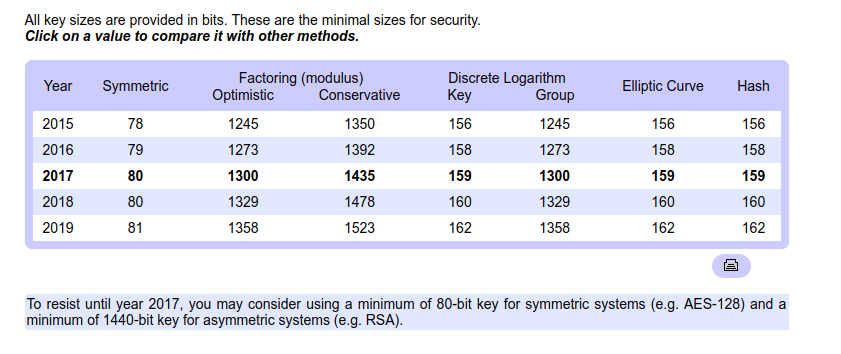
\includegraphics[width=90mm,scale=0.5]{keylengthcom.png}
  \end{figure}
\end{frame}

\begin{frame}{Влияние на рекомендации к использованию}
\begin{itemize}
\item RSA: 4096
\item DH: 2048/256
\item Elliptic curve: 512/256 (bitcoin) 
\end{itemize}

NSA не рекомендует использование алгоритмов на элиптических кривых для
внутреннего использования.
\end{frame}

\section{Заключение}
\begin{frame}{Что дальше?}
\begin{itemize}
\item Линейная алгебра (Матрицы)
\item Дискретная математика (Операции с остатком)
\end{itemize}
\end{frame}

\begin{frame}{Что дальше?}
https://github.com/ivanmurashko/lectures/tree/master/pdfs
 \begin{figure} 
   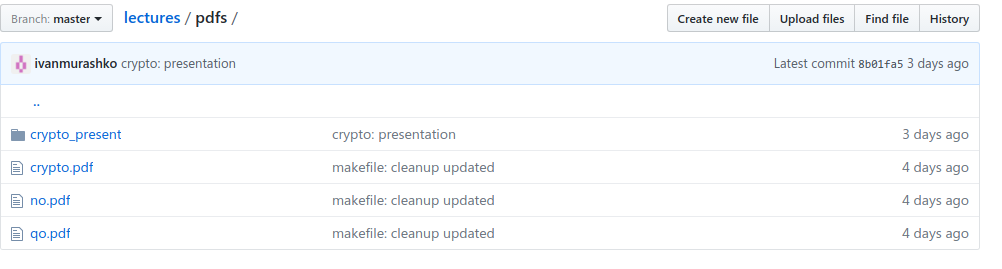
\includegraphics[width=90mm,scale=0.5]{github.png}
  \end{figure}
\end{frame}

\begin{frame}{Вопросы}
 \begin{figure} 
   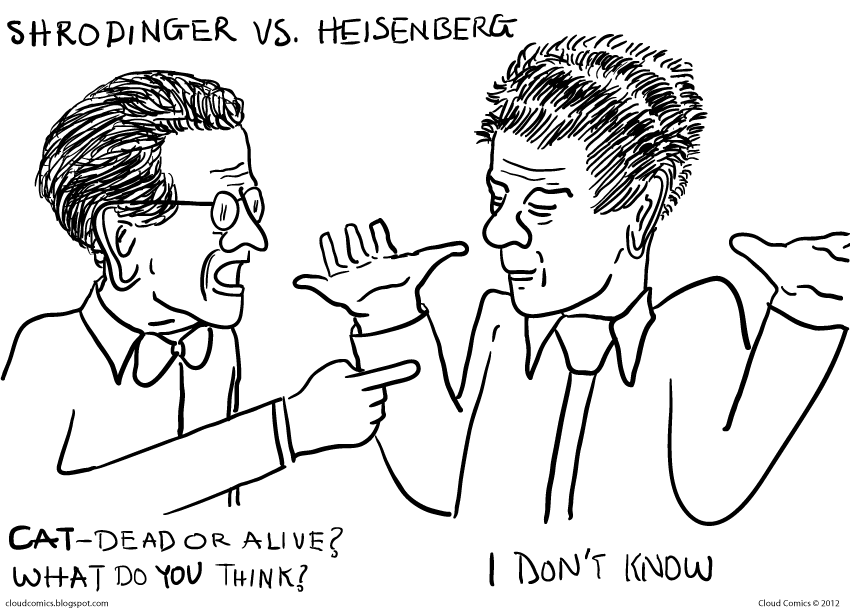
\includegraphics[width=90mm,scale=0.5]{questions.png}
  \end{figure}
\end{frame}

\end{document}
